\documentclass[a4paper,11pt]{book}
%\documentclass[a4paper,twoside,11pt,titlepage]{book}
\usepackage[pdfborder={000}, hidelinks]{hyperref} %referencia
\usepackage{listings}
\usepackage[utf8]{inputenc}
\usepackage[spanish, es-tabla]{babel}
\usepackage{eurosym}
\usepackage{csvsimple}
%\usepackage{cite}

\usepackage[loadshadowlibrary]{todonotes}
\usepackage{float, subcaption}
\usepackage{amsmath}
\usepackage{colortbl}
\usepackage{multirow}
\usepackage{multicol}
\definecolor{M1}{RGB}{255,199,2}
\usepackage{algorithm}% http://ctan.org/pkg/algorithms
\usepackage{algpseudocode}
\usepackage{rotating}
\usepackage{amsmath}
\usepackage{dirtytalk}
\usepackage{xcolor}
\usepackage{tikz}
\usepackage{makecell}

\newcommand{\code}{\lstinline}
\usepackage{dirtree}

\usepackage{csquotes}
\usepackage{microtype}
\usepackage[backend=biber, defernumbers=true, citestyle=numeric-comp, bibstyle=ieee, sorting=none]{biblatex}

\DeclareBibliographyCategory{cited}
\AtEveryCitekey{\addtocategory{cited}{\thefield{entrykey}}}
% Configurando BibLaTeX
\DefineBibliographyStrings{spanish}{
  url = {URL},
  andothers={et ~al\adddot}
}

\addbibresource{bibliografia/bibliografia.bib}

\setlength{\parindent}{0pt}

\definecolor{ugr_yellow}{rgb}{1.0, 0.78, 0}

%\usepackage[style=list, number=none]{glossary} %
%\usepackage{titlesec}
%\usepackage{pailatino}
\newcommand{\norm}[1]{\lVert#1\rVert_2}

\decimalpoint
\usepackage{dcolumn}
\newcolumntype{.}{D{.}{\esperiod}{-1}}
\makeatletter
\addto\shorthandsspanish{\let\esperiod\es@period@code}
\makeatother


%\usepackage[chapter]{algorithm}
\RequirePackage{verbatim}
%\RequirePackage[Glenn]{fncychap}
\usepackage{fancyhdr}
\usepackage{graphicx}
\usepackage{afterpage}

\usepackage{longtable}

% ********************************************************************
% Re-usable information
% ********************************************************************
\newcommand{\myTitle}{Estudio y Análisis de Metaheurísticas Modernas para el problema de la Selección de Características\xspace}
\newcommand{\myDegree}{Grado en Ingeniería Informática\xspace}
\newcommand{\myName}{Miguel García López\xspace}
\newcommand{\myProf}{Daniel Molina Cabrera\xspace}
%\newcommand{\mySupervisor}{Put name here\xspace}
\newcommand{\myFaculty}{Escuela Técnica Superior de Ingenierías Informática y de
Telecomunicación\xspace}
\newcommand{\myFacultyShort}{E.T.S. de Ingenierías Informática y de
Telecomunicación\xspace}
\newcommand{\myDepartment}{Departamento de Ciencias de la Computación e Inteligencia Artificial \xspace}
\newcommand{\myUni}{\protect{Universidad de Granada}\xspace}
\newcommand{\myLocation}{Granada\xspace}
\newcommand{\myTime}{\today\xspace}
\newcommand{\myVersion}{Version 0.1\xspace}


\hypersetup{
pdfauthor = {\myName (email (en) ugr (punto) es)},
pdftitle = {\myTitle},
pdfsubject = {},
pdfkeywords = {palabra_clave1, palabra_clave2, palabra_clave3, ...},
pdfcreator = {LaTeX con el paquete ....},
pdfproducer = {pdflatex}
}
%\hyphenation{}


%\usepackage{doxygen/doxygen}
%\usepackage{pdfpages}
\usepackage{url}
\usepackage{colortbl,longtable}
\usepackage[stable]{footmisc}
%\usepackage{index}
\usepackage{booktabs} % Required for \bottomrule
\usepackage{adjustbox}
\usepackage{pdflscape}
\usepackage{changepage}

%\makeindex
%\usepackage[style=long, cols=2,border=plain,toc=true,number=none]{glossary}
%\makeglossary

% Definición de comandos que me son tiles:
%\renewcommand{\indexname}{Índice alfabético}
%\renewcommand{\glossaryname}{Glosario}

\pagestyle{fancy}
\fancyhf{}
\fancyhead[LO]{\leftmark}
\fancyhead[RE]{\rightmark}
\fancyhead[RO,LE]{\textbf{\thepage}}
\renewcommand{\chaptermark}[1]{\markboth{\textbf{#1}}{}}
\renewcommand{\sectionmark}[1]{\markright{\textbf{\thesection. #1}}}

\setlength{\headheight}{1.5\headheight}

\newcommand{\HRule}{\rule{\linewidth}{0.5mm}}
%Definimos los tipos teorema, ejemplo y definición podremos usar estos tipos
%simplemente poniendo \begin{teorema} \end{teorema} ...
\newtheorem{teorema}{Teorema}[chapter]
\newtheorem{ejemplo}{Ejemplo}[chapter]
\newtheorem{definicion}{Definición}[chapter]

\definecolor{gray97}{gray}{.97}
\definecolor{gray75}{gray}{.75}
\definecolor{gray45}{gray}{.45}
\definecolor{gray30}{gray}{.94}

\lstset{ frame=Ltb,
     framerule=0.5pt,
     aboveskip=0.5cm,
     framextopmargin=3pt,
     framexbottommargin=3pt,
     framexleftmargin=0.1cm,
     framesep=0pt,
     rulesep=.4pt,
     backgroundcolor=\color{gray97},
     rulesepcolor=\color{black},
     %
     stringstyle=\ttfamily,
     showstringspaces = false,
     basicstyle=\normalsize\ttfamily,
     commentstyle=\color{gray45},
     keywordstyle=\bfseries,
     %
     numbers=left,
     numbersep=6pt,
     numberstyle=\tiny,
     numberfirstline = false,
     breaklines=true,
   }
 
% minimizar fragmentado de listados
\lstnewenvironment{listing}[1][]
   {\lstset{#1}\pagebreak[0]}{\pagebreak[0]}

\lstdefinestyle{CodigoC}
   {
	basicstyle=\scriptsize,
	frame=single,
	language=C,
	numbers=left
   }
\lstdefinestyle{CodigoC++}
   {
	basicstyle=\small,
	frame=single,
	backgroundcolor=\color{gray30},
	language=C++,
	numbers=left
   }

 
\lstdefinestyle{Consola}
   {basicstyle=\scriptsize\bf\ttfamily,
    backgroundcolor=\color{gray30},
    frame=single,
    numbers=none
   }


\newcommand{\bigrule}{\titlerule[0.5mm]}


%Para conseguir que en las páginas en blanco no ponga cabecerass
\makeatletter
\def\clearpage{%
  \ifvmode
    \ifnum \@dbltopnum =\m@ne
      \ifdim \pagetotal <\topskip
        \hbox{}
      \fi
    \fi
  \fi
  \newpage
  \thispagestyle{empty}
  \write\m@ne{}
  \vbox{}
  \penalty -\@Mi
}
\makeatother

\usepackage{pdfpages}

% % Temporarly
% \usepackage{fancyhdr}
% \pagestyle{fancyplain}
% \fancyhead{}
% \lfoot{\scriptsize\LaTeX}
% \cfoot{\hyperlink{listoftodos}{ToDoList} || \hyperlink{tableofcontents}{TableOfContents}}
% \rfoot{\small\thepage}

\begin{document}
\begin{titlepage}
 
 
\newlength{\centeroffset}
\setlength{\centeroffset}{-0.5\oddsidemargin}
\addtolength{\centeroffset}{0.5\evensidemargin}
\thispagestyle{empty}

\noindent\hspace*{\centeroffset}\begin{minipage}{\textwidth}

\centering

\includegraphics[width=0.9\textwidth]{imagenes/UGR-MARCA-02-color.png}\\[1.4cm]

\textsc{ \Large TRABAJO FIN DE GRADO\\[0.2cm]}
\textsc{ INGENIERÍA INFORMÁTICA}\\[1cm]
% Upper part of the page
% 
% Title
{\Huge\bfseries Estudio y Análisis de Metaheurísticas modernas para el problema de Selección de Características\\
}
\noindent\rule[-1ex]{\textwidth}{3pt}\\[3.5ex]
\end{minipage}

\vspace{1.4cm}
\noindent\hspace*{\centeroffset}\begin{minipage}{\textwidth}
\centering

\textbf{Autor}\\ {Miguel García López}\\[2.5ex]
\textbf{Directores}\\
{Daniel Molina Cabrera}\\[2cm]

\includegraphics[width=0.3\textwidth]{imagenes/etsiit_logo.png}\\[0.1cm]
\textsc{Escuela Técnica Superior de Ingenierías Informática y de Telecomunicación}\\
\textsc{---}\\
Granada, Enero de 2024
\end{minipage}
%\addtolength{\textwidth}{\centeroffset}
%\vspace{\stretch{2}}
\end{titlepage}


\begin{frame}[plain]
  
  \titlepage

  
  \begin{tikzpicture}[overlay,remember picture]
      \node[left=-0.30cm] at (current page.0){
          
\includegraphics[scale=0.142]{imagenes/IntroBackground}
      };
  \end{tikzpicture}
\end{frame}

\note{
Mi nombre es Miguel García López, estudiante del Grado de Ingeniería Informática. Hoy presento mi proyecto de TFG, gracias a la tutorización del profesor Daniel Molina Cabrera. En esta presentación, se explicará el problema de selección de características y la aplicación de metaheurísticas al mismo. Se realizará un estudio y análisis de varias versiones y varios algoritmos.
}

\begin{frame}[noframenumbering]
    \frametitle{Índice}
  \begin{multicols}{2}
  \tableofcontents
  \end{multicols}
\end{frame}


\frontmatter
\mainmatter

\tableofcontents
\listoffigures
\listoftables
\setlength{\parskip}{5pt}

\chapter{Introducción}
\section{Definición del problema}
El problema de la selección de características se define como el proceso de
seleccionar un subconjunto de características relevantes~\cite{miao_survey_2016}. Una característica es
una propiedad individual medible de un fenómeno concreto. Este problema es
considerado un problema \textbf{NP duro}. La reducción de dimensionalidad, y con
ello de características, suele ser necesario a la hora de crear un modelo predictivo por medio
del aprendizaje automático ya que muchas de las características
dentro de un conjunto de datos pueden no llegar a ser relevantes para solucionar
aquellos problemas que se intentan solucionar, ya sea por que no aporta información,
porque puede ser agrupada junto a otras tantas en una sola propiedad o incluso porque hay ruido
en los datos, lo cual es inevitable~\cite{Mostafa2012}.\\[6pt]
Gracias a la reducción de características es posible mejorar tanto la capacidad de generalización
como la precisión del modelo predictivo gracias a la reducción de \textit{ruido}.\\[6pt]
Siendo $f$ la función objetivo a predecir, $H^n$ el conjunto de hipótesis o conjunto de modelos
de dimensión $n$ posibles, $h^*(x)$ el mejor modelo aprendido y $x$ una variable de entrada. El ruido conocido
como ruido estocástico es aquel que atiende a una variación aleatoria que
puede surgir de diversos factores, como mediciones imprecisas de señales o la falta de
precisión en sensores. Por otro lado, el ruido determinista está directamente
relacionado con la complejidad de un modelo. Su presencia aumenta la probabilidad de
sobreajuste. El ruido determinista puede explicarse como la parte de la función $f$ que el conjunto
de hipótesis $H^n$ no puede capturar, es decir, $f(x) - h^*(x)$. Este tipo de ruido se
considera así porque la función (modelo) no es lo suficientemente compleja como para comprender
esa parte. Este ruido depende de $H^n$ y permanece constante para un valor dado de $x$~\cite{Mostafa2012}.\\[6pt]
La reducción de características ayuda a manejar ambos tipos de ruido~\cite{miao_survey_2016,Mostafa2012} al simplificar el
modelo, lo que puede reducir el impacto del ruido estocástico y disminuir la complejidad del
modelo, lo que a su vez puede ayudar a mitigar el ruido determinista al mejorar la capacidad
del modelo para capturar las características relevantes y descartar las irrelevantes.
Esto puede conducir a una mejor capacidad de generalización y a una reducción del sobreajuste.\\[6pt]
Además de la simplificación del modelo, que conduce a una reducción del ruido, la
selección de características es un preprocesamiento necesario por varias razones:
\begin{enumerate}
      \item Interpretabilidad: La presencia de características
            irrelevantes puede complicar innecesariamente la interpretación y el
            rendimiento de los modelos de aprendizaje automático~\cite{miao_survey_2016}. La selección de un
            subconjunto relevante de características puede simplificar el modelo
            resultante, haciéndolo más comprensible y fácilmente interpretable.

      \item Mejora de la eficiencia computacional: La reducción de la
            dimensionalidad puede conducir a un ahorro significativo en términos de
            tiempo y recursos computacionales necesarios para el entrenamiento y la
            evaluación de modelos. Al eliminar características irrelevantes, se reduce
            la complejidad del problema y se acelera el proceso de aprendizaje.

      \item Evita la maldición de la dimensionalidad: Cuando la dimensionalidad
            se incrementa en un problema, el volumen del espacio también lo hace, y esto ocurre
            tan rápido que  hace que los datos disponibles se vuelvan dispersos. De forma que para
            obtener un resultado seguro/fiable, la cantidad de datos necesitados debe verse
            incrementada de manera exponencial con la dimensionalidad~\cite{udacity2015curse}. A menor dimensionalidad
            (características en el conjunto de datos) menos datos harán falta para obtener un buen
            modelo.
\end{enumerate}
En este trabajo, se lleva a cabo una investigación y análisis comparativo entre varios métodos
de la familia \textbf{wrapper} o métodos de envoltura. Existen multitud de estrategias~\cite{miao_survey_2016}
que intentan dar solución a este problema. Los métodos de búsqueda más famosos son los de filtrado
(\textbf{filter}), los cuáles seleccionan las características más discriminativas según la naturaleza de los datos~\cite{miao_survey_2016}.
Por lo general, estos métodos realizan la selección de características antes de las tareas de clasificación y
agrupamiento. Ejemplos de algoritmos de filtrado son \textit{relieF}~\cite{kira_practical_1992} o F-statistic~\cite{ding_minimum_2005}.\\[6pt]
Los métodos \textbf{wrapper}, en cambio, utilizan el algoritmo de aprendizaje usado postprocesamiento
para evaluar las características y seleccionar así las más útiles~\cite{miao_survey_2016}.\\[6pt]
Los algoritmos clasificatorios de aprendizaje utilizados en este trabajo son \textit{SVM}~\cite{cortes_support-vector_1995}
y \textit{kNN}~\cite{fix_discriminatory_1989,cover_nearest_1967}, siendo las máquinas de vectores de
soporte un método robusto y eficiente y los vecinos más cercanos un método simple, interpretable
y muy eficaz. Se analizará el resultado entre ambos clasificadores entre otros muchos análisis comparativos.

\subsection{Motivación}
El reciente interés del problema de la selección de características en el ámbito de las
metaheurísticas en los últimos años es más que evidente. Puede comprobarse como en los
últimos años hay una tendencia en la publicación de artículos presentando nuevos métodos
metaheurísticos, mejores con respecto a los clásicos o incluso comparativas y análisis entre
distintos algoritmos.\\[6pt]

Esta crecimiento viene acompañado, sin embargo, de comparaciones que distan de ser objetivas
por varios motivos. Entre varios artículos se comparan algoritmos del mismo tipo con
soluciones y resultados muy variables entre sí a pesar de mismas configuraciones a la hora
de experimentar, artículos sin código referenciado, de forma que sea más fácil interpretar
los resultados o duplicarlos, y algoritmos novedosos presentados por su autor o autores que
superanmal resto en alguna métrica concreta sin llegar a la rigurosidad adecuada.\\[6pt]

Por ello, la motivación principal de este trabajo es la de proveer información no sesgada y
todo lo objetiva posible por medio de un análisis comparativo entre los
algoritmos optimizatorios metaheurísticos más populares y más citados junto con los
algoritmos más robustos y clásicos en el campo de la optimización pseudo estocástica.

\subsection{Objetivos}
\textbf{Objetivo General:}

Realizar una comparación exhaustiva y objetiva de diversas metaheurísticas utilizadas en la
selección de características, con el propósito de proporcionar una visión integral y
evaluativa sobre su eficacia y aplicabilidad en diferentes contextos de análisis de
datos.\\[6pt]
\textbf{Objetivos Específicos:}

\begin{enumerate}
      \item Evaluar el desempeño de las metaheurísticas más relevantes en el ámbito de la
            selección de características, analizando métricas clave como precisión, estabilidad de
            las soluciones y eficiencia computacional. Se emplearán conjuntos de datos de referencia
            y metodologías de validación cruzada para garantizar la robustez de los resultados.

      \item Investigar la transferibilidad de las técnicas diseñadas para dominios continuos y
            binarios en el contexto de la selección de características. Se analizará si las
            metaheurísticas efectivas en un dominio son igualmente eficaces cuando se aplican a
            otro, identificando posibles ventajas y limitaciones de cada enfoque.

      \item Identificar las fortalezas y debilidades de cada metaheurística según el tipo de
            representación de las características. Se realizará un análisis detallado del
            comportamiento de las técnicas en problemas de selección de características con
            diferentes tipos de datos, destacando su rendimiento relativo y sus áreas de aplicación
            más adecuadas.

      \item Proporcionar recomendaciones prácticas basadas en los resultados obtenidos, con el
            objetivo de orientar a practicantes y académicos en la selección y aplicación de
            metaheurísticas en problemas reales de selección de características.

      \item Evaluar los resultados de las metaheurísticas en problemas de selección de característica
            usando distintos como algoritmos de aprendizaje los métodos \textit{kNN} y \textit{SVM}. Se realizará
            una comparativa a nivel de eficiencia en tiempo, estabilidad y calidad de los resultados.
\end{enumerate}

\subsection{Planificación}
Un trabajo de fin de grado consta de $12$ créditos ECTS, donde se estima que cada crédito debe valer unas $25$ horas de trabajo aproximadamente. Teniendo en cuenta estos datos, se calcula que la duración del TFG no debería ser superior a $300$ horas. Ha de tenerse en cuenta también que el alumno trabaja $25$ horas semanales y debe superar algunas asignaturas además de su projecto final para terminar la carrera. Por lo tanto, el proyecto se planifica con una duración extendida en el tiempo, pero con una carga de trabajo semanal menos intensiva.\\[6pt]
Se planifica una duración de $5$ meses aproximadamente. Se utilizará un diagrama de Gantt~\cite{Clark1922} para describir la planificación del proyecto, de manera que se realizarán tareas en un orden cronológico. Sin embargo, se reconoce que algunas tareas probablemente requerirán iteraciones posteriores, ya que es probable que se mejore y perfeccione el proyecto a lo largo de su ciclo de vida.\\[6pt]
Las fases del ciclo de vida son:
\begin{itemize}
      \item \textbf{Investigación inicial}
            Esto incluye investigar sobre conceptos básicos ya aprendidos, en forma de repaso sobre conceptos generales de aprendizaje automático, tipos de metaheurísticas, tipos de codificación, optimización de funciones, test estadísticos y conceptos básicos, código Python y librerías asociadas, instalación de estas a partir de un entorno virtual, configuración del entorno de trabajo e investigación sobre el problema de selección de características.

      \item \textbf{Diseño del software}: Planificación de la estructura general del código, uso de patrones de diseño que puedan ser de utilidad de cara a al mantenimiento del software a lo largo del desarrollo, concepto de modularización inicial del código (estructura del proyecto), uso de entornos virtuales.
      \item \textbf{Investigación metaheurísticas}: Realización de un estudio más exhaustivo acerca de las metaheurísticas a implementar y sus diferentes versiones binarias. Esto incluye un listado de 12 metaheurísticas, siendo estas:
            \begin{itemize}
                  \item Binary Firefly Algorithm
                  \item Binary Whale Optimization Algorithm
                  \item Binary Bat Swarm Optimizer
                  \item Binary Grey Wolf Optimizer
                  \item Binary Dragonfly Algorithm
                  \item Binary Grasshoper Algorithm
                  \item Binary Cuckoo Search
                  \item Binary Differential Algorithm
                  \item Ant Colony Optimization
                  \item Binary Artificial Bee Colony Optimization
                  \item Binary Particle Swarn Optimization
                  \item Genetic Algorithm (binary \& real)
            \end{itemize}
            De cada una de ellas se investigará su inspiración, funcionamiento, implementación y versiones binarias, normalmente asociadas al problema de selección de características.
      \item \textbf{Implementación del software}: Una vez claros los requisitos programáticos quedan establecidos, se implementará el software base. Esto incluye código en Python para la generación de gráficas, manejo de datasets en formato \textit{arff}, codificación de los algoritmos metaheurísticos en versión binaria, implementación de función objetivo (\textit{fitness}) y parametrización del programa para distintas pruebas.
      \item \textbf{Pruebas y refactorizado}: En esta etapa se llevarán a cabo pruebas exhaustivas para verificar la robustez y eficacia de los diferentes algoritmos implementados. Además, se considerará la refactorización del código si es necesario, con el fin de mejorar su estructura, claridad y mantenibilidad. 
      \item \textbf{Análisis de resultados}: En esta fase se recopilarán datos de la ejecución de los algoritmos en sus diferentes versiones, así como entre ellos, utilizando los conjuntos de datos seleccionados para el proyecto. Esta recopilación de métricas permitirá una evaluación del rendimiento y la eficacia de cada algoritmo en comparación con los demás, así como su comportamiento en diferentes conjuntos de datos.
      \item \textbf{Documentación}: En esta etapa final se generará una documentación del proyecto que incluirá de forma general la descripción del problema, los objetivos, planificación, implementación, resultados y pruebas.
\end{itemize}

\begin{figure}[H]
      \begin{center}
      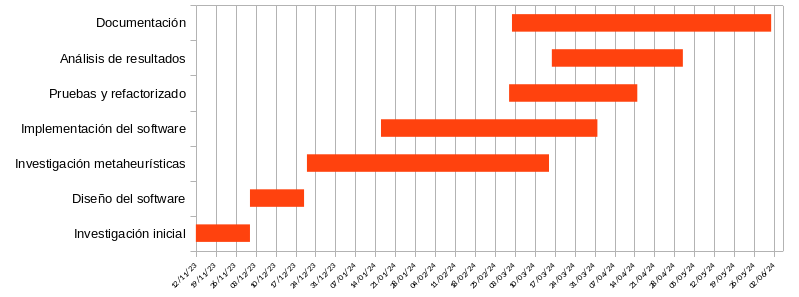
\includegraphics[width=1.2\textwidth]{imagenes/gantt-init.png}
      \end{center}
      \caption{Diagrama de Gantt inicial}
\end{figure}

La planificación inicial tiene en cuenta un curso ideal del ciclo de vida del proyecto, siendo las estapas más extensas la de creación del software e implementación de la documentación. Son etapas excluyentes, no pueden ocurrir a la vez según este tipo de planificación. Al terminar una etapa se pasa inmediatamente a la siguiente.\\[6pt]
La planificación final del proyecto se ha modificado significativamente debido a una serie de contratiempos y obstáculos surgidos durante su desarrollo, así como la influencia de numerosos eventos externos que han afectado a su cronograma. En particular, se han experimentado retrasos y bloqueos que han incidido en la duración prevista del proyecto. Por ejemplo, las etapas de implementación del software y la investigación de las metaheurísticas se han entrelazado debido a que la implementación efectiva del algoritmo se facilitaba una vez que se había estudiado a fondo la metaheurística correspondiente. Esto ha llevado a una reevaluación de la estrategia de planificación original, reconociendo que no habría sido eficiente estudiar todas las metaheurísticas simultáneamente y luego proceder con su implementación.

\begin{figure}[H]
      \begin{center}
      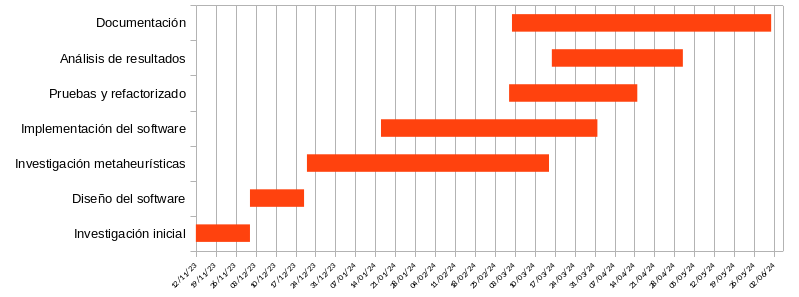
\includegraphics[width=1.2\textwidth]{imagenes/gantt-init.png}
      \end{center}
      \caption{Diagrama de Gantt final}
\end{figure}

El coste estimado del proyecto se divide en varios subcostes:
\begin{itemize}
      \item \textbf{Sueldo}: Teniendo en cuenta que el sueldo medio en España para un científico de datos es de $39.000$€~\cite{payscale_barcelona} al año y que el proyecto consta de un solo trabajador, se puede estimar un salario de $18.75$€/hora. 
\end{itemize}
\input{capitulos/02_Planificación}
\chapter{Fundamentos Teóricos}
En este capítulo se describirán aquellos conceptos teóricos fundamentales para comprender el trabajo realizado en este proyecto.

\section{Optimización}
La optimización es un campo de estudio que trata, mediante el uso de las adecuadas herramientas matemáticas, de maximizar o minimizar una función objetivo. Esto significa, obtener la mejor solución posible para un problema dado dentro de un conjunto de alternativas y normalmente sujeto a una serie de restricciones que hacen de una solución satisfacible. Es un área interdisciplinar que aborda desde campos tales como la Economía, Ingeniería, Biología y muchas otras tantas disciplinas.\\[6pt]
La optimización es una disciplina arraigada en la naturaleza humana. Este impulso innato hacia la optimización ha llevado al desarrollo de diversas metodologías y técnicas a lo largo de la historia, desde los rudimentarios métodos de prueba y error hasta los sofisticados algoritmos de optimización computacional utilizados en la actualidad.

\subsection{Definición general de un problema de optimización}
Para poder convertir un problema abstracto en un problema de optimización concreto, con el que se pueda trabajar, es necesario establecer ciertos elementos fundamentales que lo definan de manera precisa y clara. En general, un problema de optimización se expresa de la siguiente forma~\cite{inbook}:

\begin{subequations}
    \begin{alignat}{2}
         & \text{Función objetivo a minimizar}                       & \qquad & f(x)\label{eq:optProb}                             \\
         & \text{Sujeto a} \nonumber                                                                                               \\
         & s \text{ restricciones de desigualdad}                    & \qquad & g_i(x)\leq 0, \quad j=1,2,...,s\label{eq:optProb2} \\
         & w \text{ restricciones de igualdad}                       & \qquad & h_j(x) = 0, \quad j=1,2,...,w\label{eq:optProb3}   \\
         & \text{Donde el número de variables es dado por} \nonumber & \qquad & x_i, \quad i=1,2,...,n
    \end{alignat}
\end{subequations}

La definición general de un problema de optimización proporciona una estructura sólida para abordar el problema abstracto. Establece la función objetivo que se busca minimizar o maximizar, junto con las restricciones que deben cumplirse. Estas restricciones pueden ser tanto desigualdades como igualdades, y todas juntas definen el \textbf{espacio de búsqueda} del problema.

\subsection{Función objetivo y función fitness}
Ambos términos, aunque a menudo se utilizan como sinónimos, desempeñan roles distintos en el ámbito de la optimización. La función \textit{objetivo}, como su nombre indica, establece el objetivo a alcanzar en la resolución del problema. Esta función cuantifica el rendimiento de las soluciones encontradas en relación con el objetivo específico del problema, que puede ser maximizar ganancias, minimizar distancia, entre otros objetivos. Por otro lado, la función de \textit{fitness} solo tiene que evaluar la idoneidad de una solución dentro de una población de soluciones. Es decir, determina la calidad relativa de la solución respecto a otras alternativas.

Por otro lado, la función objetivo puede ser positiva o negativa, dependiendo de si se busca maximizar o minimizar el objetivo. Además, la función \textit{fitness} también puede llegar a ser una aproximación de la función objetivo, pero no necesariamente coinciden exactamente.\\[6pt]
Resumiendo, la función \textit{fitness} es un tipo particular de función objetivo que se utiliza como métrica de rendimiento~\cite{eiben2015}.

\subsection{Óptimos globales o locales}
Se conocen como punto de óptimo global (mínimo o máximo) la solución (o vector hablando en términos matemáticos) cuyo valor para la función objetivo es el más grande en todo el espacio de soluciones posible, es decir, el espacio de búsqueda. Los óptimos locales en cambio son varios, no solo uno como es el global. Son soluciones máximas o mínimas dentro de una región de soluciones.

\begin{figure}[H]
    \begin{center}
        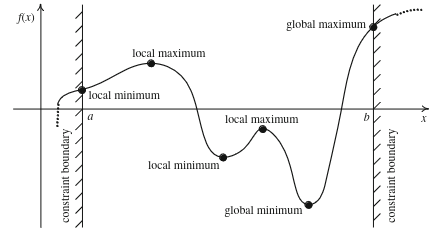
\includegraphics[width=1\textwidth]{imagenes/min-max_points.png}
    \end{center}
    \caption[Puntos globales y locales]{En esta figura extraída de \cite{inbook} puede observarse de manera intuitiva la diferencia entre punto global y puntos locales. El máximo global es el valor más alto para $f(x)$ en el espacio, mientras que un máximo global solo representa el valor más alto dentro de un ``vecindario"}
\end{figure}

Sea $f(x)$ una función a maximizar y $x^*$ una solución óptima. Un objetivo $G(x)$ está en su máximo global sí y solo si~\cite{inbook}:
\begin{equation}
    f(x^*) \geq f(x) \quad \forall x
\end{equation}
En cambio el objetivo está en un máximo local en el punto $x^*$ si:
\begin{equation}
    \begin{split}
        f(x^*) \geq f(x) \quad & \forall x \\
        & \text{dentro de un vecindario de } x^*\text{~\cite{inbook}}
    \end{split}
\end{equation}

\section{Selección de características}
La selección de características es un ejemplo de problema $NP$-Hard y uno de los problemas más importantes en el mundo de la inteligencia artificial, más concretamente en el \textbf{machine learning} o aprendizaje automático.

\subsection{Necesidad y motivo}
El aprendizaje automático se basa en los datos como fuente de aprendizaje. Es indispensable tener un buen conjunto de datos para poder obtener un modelo robusto y preciso. Por norma general o como se diría en inglés \textit{``as a rule of thumb''}, a más grande el conjunto de datos, mayor calidad del modelo. De hecho hay una correlación inmediata con esta sentencia.

\begin{figure}[H]
    \begin{center}
        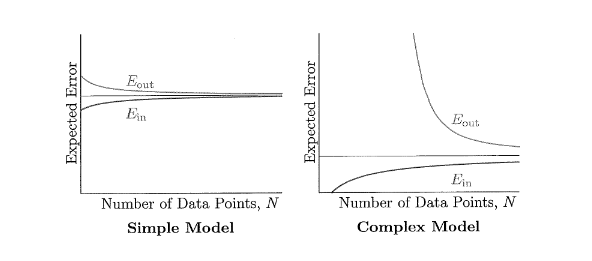
\includegraphics[width=1\textwidth]{imagenes/learning_from_data_vc.png}
    \end{center}
    \caption[Correlación entre error del modelo y N]{Esta figura extraída de \cite{Mostafa2012} visualiza la relación directa entre calidad del modelo (menos error esperado) y número de datos que se le proporciona al algoritmo de aprendizaje.}
    \label{fig:learning_from_data_vc}
\end{figure}

Es inmediato pensar que, a mayor cantidad de datos, mejor calidad del modelo, y así suele ser. Sin embargo, también existe una ``normal general'' que relaciona la complejidad del modelo y su capacidad de generalización. Es cierto que un modelo muy complejo (muchos parámetros) es capaz de ajustar mejor funciones más complejas, pero dentro de un conjunto con una serie de modelos suficientemente complejos, suele ser mejor idea elegir el más simple. Hay una serie clara de ventajas para ello:
\begin{enumerate}
    \item Menor  sensibilidad al sobre-ajuste.
    \item Mayor interpretabilidad del modelo y sus resultados.
    \item Mayor eficiencia y por tanto menor tiempo de ejecución y menor peso en memoria.
\end{enumerate}

De hecho, como puede observarse en la figura \ref{fig:learning_from_data_vc}, el modelo más complejo tiene un error esperado mucho mayor que el simple. El $E_{out}$ o error fuera de la muestra (error de generalización) es mucho más abrupto, es decir, generaliza peor.\\[6pt]
Por supuesto, con suficientes datos, con un $N$ (número de datos) suficientemente grande, la tendencia del error es a la baja~\cite{Mostafa2012, shalev2014understanding}. Ocurre, sin embargo, que la recolección, limpieza y transformación de datos es una tarea compleja, por ello es mejor ceñirse, de nuevo, a el modelo más pequeño que obtenga una solución con suficiente calidad.\\[6pt]

Como se ha mencionado anteriormente, la selección de características ayuda a la reducción del ruido. Siendo $f$ la función objetivo a predecir, $H^n$ el conjunto de hipótesis o conjunto de modelos de dimensión $n$ posibles, $h^*(x)$ el mejor modelo aprendido y $x$ una variable de entrada. El ruido conocido
como ruido estocástico es aquel que atiende a una variación aleatoria que
puede surgir de diversos factores, como mediciones imprecisas de señales o la falta de
precisión en sensores. Por otro lado, el ruido determinista está directamente
relacionado con la complejidad de un modelo. Su presencia aumenta la probabilidad de
sobre-ajuste. El ruido determinista puede explicarse como la parte de la función $f$ que el conjunto
de hipótesis $H^n$ no puede capturar, es decir, $f(x) - h^*(x)$. Este tipo de ruido se
considera así porque la función (modelo) no es lo suficientemente compleja como para comprender
esa parte. Este ruido depende de $H^n$ y permanece constante para un valor dado de $x$~\cite{Mostafa2012}.\\[6pt]
La reducción de características ayuda a manejar ambos tipos de ruido~\cite{miao_survey_2016,Mostafa2012} al simplificar el
modelo, lo que puede reducir el impacto del ruido estocástico y disminuir la complejidad del
modelo, lo que a su vez puede ayudar a mitigar el ruido determinista al mejorar la capacidad
del modelo para capturar las características relevantes y descartar las irrelevantes.
Esto puede conducir a una mejor capacidad de generalización y a una reducción del sobre-ajuste.\\[6pt]

\subsection{Concepto}
El funcionamiento y motivo es explicado ya en la sección de motivación en \ref{motivation}. Por evitar redundancias se procede a explicar el concepto de manera abreviada y puntualizando en los apartados más importantes.\\[6pt]
La selección de características es una conocida y necesaria técnica de pre-procesamiento de datos para la construcción de un modelo de aprendizaje. Su función es escoger un subconjunto óptimo de características dentro del conjunto inicial, de forma que la complejidad del modelo se reduzca.\\[6pt]
Este problema es del tipo $NP$-Hard, como ya se ha mencionado previamente en \ref{motivation} y explicado en \ref{complexity}.
La selección de características ayuda a una serie de factores como son la interpretabilidad, mejora de la eficiencia temporal y espacial del modelo y sobre todo con la \textbf{maldición de la dimensionalidad}~\cite{venkat2018curse, bellman1957dynamic}.

\subsection{Maldición de la dimensionalidad}
El término fue acuñado por Bellman en $1961$~\cite{bellman1961adaptive}. Este fenómeno ocurre cuando la dimensionalidad de los datos es muy grande. En un espacio de características de alta dimensión, es común que los datos estén muy dispersos, lo que significa que hay muy pocos datos en comparación con la cantidad posible de características. Esto dificulta que los modelos representen correctamente todo el espacio de características~\cite{peng_interpreting_2024}.

\begin{figure}[H]
    \begin{center}
        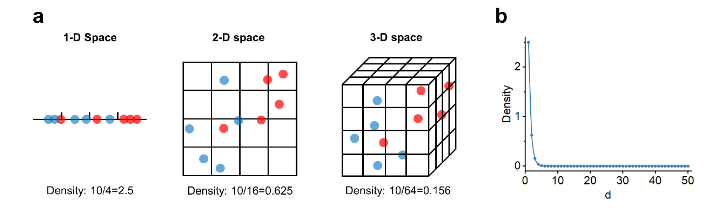
\includegraphics[width=1\textwidth]{imagenes/curse-dimen-example.png}
    \end{center}
    \caption[Tendencia de incremento de dimensionalidad en varios espacios de características]{Esta figura extraída de \cite{peng_interpreting_2024} muestra la tendencia en la densidad a medida que se incrementa la dimensionalidad del espacio. En $(a)$ se muestra la densidad con diez puntos de datos en un espacio $1D$, en $(b)$ se muestra la tendencia al incrementar las dimensiones.}
\end{figure}

Además, en espacios de alta dimensión, la medición de distancias puede volverse menos precisa. Esto se debe a que las distancias entre puntos de datos diferentes tienden a converger a un mismo valor a medida que aumenta la dimensionalidad. Esto significa que las medidas de distancia ya no son tan útiles para medir la similitud entre datos~\cite{peng_interpreting_2024, venkat2018curse}. En el trabajo de Beyer y colaboradores~\cite{beyer99nn} se observó como esto ocurría y por tanto un escaneo lineal (recorrer los puntos uno a uno) resultaba en altas dimensiones más práctico que otras técnicas complejas.
\section{Metaheurísticas}
Dentro de la optimización hay muchos tipos de métodos, dentro de los pseudoaleatorios pueden encontrarse las metaheurísticas. Estas son algoritmos basados en una abstracción de mayor nivel de la \textbf{heurísticas}. Mientras que las heurísticas se apoyan en el conocimiento específico del campo en el que se encuentra el problema, y están restringidas a su dominio, las metaheurísticas son aplicables a todo tipo de problemas, independientemente de su área de optimización~\cite{bianchi2009survey}. Es cierto que hay algoritmos que son más convenientes para ciertos problemas que otros, pero su aplicación es generalizada. Normalmente, las metaheurísticas son diseñadas a siguiendo una inspiración en la naturaleza, ya sea en fenómenos físicos o en el comportamiento animal. Ejemplo de estos son algoritmos como el \textit{Búsqueda Cuckoo}, \textit{Enfriamiento Simulado} o incluso \textit{Algoritmos Genéticos}.\\[6pt]
Las metaheurísticas son especialmente útiles en problemas cuya resolución no es factible debido a altos costos computacionales, ya sea porque es posible analíticamente pero computacionalmente costoso, o porque el problema no es abordable mediante algoritmos convencionales. Son capaces de encontrar óptimos locales lo suficientemente aceptables, soluciones no óptimas, pero si muy buenas~\cite{bianchi2009survey}.

\begin{figure}[H]
    \begin{center}
        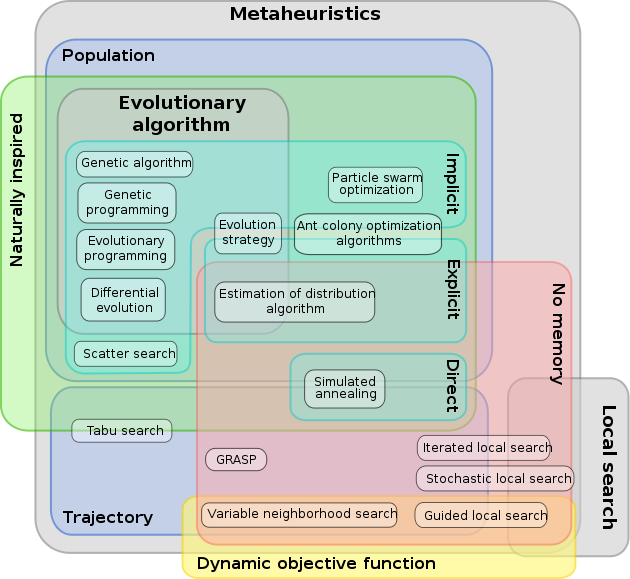
\includegraphics[width=0.8\textwidth]{imagenes/mh_euler_graph.png}
    \end{center}
    \caption[Clasificación metaheurísticas]{En esta figura de los autores Johann ``nojhan'' Dréo y Caner Candan, se clasifican las distintas metaheurísticas por inspiración.}
\end{figure}

\subsection{Exploración vs explotación}
Las metaheurísticas, y algoritmos basados en técnicas pseudoaleatorias, deben tener un balance entre sus factores explorativos y explotativos. De no ser así, los algoritmos tendrían tendencias a la convergencia temprana, dejando de lado mucho espacio por explorar y por ende soluciones posiblemente mejores (estancamiento en óptimos locales) o serían muy lentos en la convergencia hacia una solución.\\[6pt]
La \textbf{exploración} se refiere a la habilidad del algoritmo de buscar nuevas y diversas regiones en el espacio de búsqueda/solución. Es una característica de la búsqueda global, que también puede ser llamada \textit{diversificación}. En cambio, la \textbf{explotación} es la habilidad de la búsqueda de explotar las mejores soluciones encontradas hasta el momento y mejorarlas localmente, dentro de un ``vecindario''~\cite{xu2014exploration}.\\[6pt]
No existe un equilibrio \textit{de facto} entre exploración y explotación en las metaheurísticas. Aún no se ha alcanzado una respuesta definitiva a esta cuestión. Desde una perspectiva de sistemas, una metaheurística puede entenderse como un sistema dinámico compuesto por numerosos ``individuos'' que interactúan entre sí. Estos individuos representan las distintas soluciones o posiciones en el espacio de búsqueda que la metaheurística explora~\cite{6896450}. Las interacciones entre estos individuos son las que conforman comportamientos explorativos o explotativos y dependen del problema a solucionar y del propio algoritmo su equilibrio.

\section{Teorema No Free Lunch}\label{sec:teorema-no-free-lunch}
El Teorema de ``No Free Lunch'' (NFL) establece que, en promedio, ningún algoritmo de búsqueda puede superar a otros algoritmos en la búsqueda de todas las funciones objetivo posibles. En otras palabras, no existe un algoritmo universalmente óptimo que pueda dominar en todos los problemas de búsqueda. Esto implica que, si un algoritmo es efectivo para un conjunto particular de problemas, es probable que no lo sea para otros~\cite{585893}.\\[6pt]
Relacionar este teorema con las metaheurísticas implica reconocer que no hay una única metaheurística que sea la mejor para todos los problemas de optimización. Cada problema puede tener características únicas que lo hacen más o menos adecuado para ciertas metaheurísticas. Por lo tanto, en lugar de buscar una solución universal, las metaheurísticas se centran en explorar y explotar diferentes áreas del espacio de búsqueda para encontrar soluciones aceptables o incluso óptimas para problemas específicos.\\[6pt]
Pese a ello, las suposiciones de este tipo de teoremas, como conjuntos de datos extraídos de una distribución uniforme sobre todos los conjuntos de datos posibles, están completamente desalineadas con el mundo real, donde los datos suelen ser altamente estructurados y no están uniformemente muestreados~\cite{goldblum2023free}.\\[6pt]
De esta forma y faltando evidencia concluyente al respecto, es interesante mencionar el \textbf{NFL}, pero sin llegar a negar la posibilidad de nuevas y más precisas interpretaciones.

\section{Aprendizaje automático}
El aprendizaje automático es una sub-rama de estudio de la inteligencia artificial o \textbf{IA}, la cual aglomera una serie de métodos que pueden, de manera automática, detectar patrones en conjuntos masivos de datos para predecir datos futuros~\cite{murphy2012machine}. El aprendizaje automático o \textit{machine learning} en inglés, es usado en una amplia variedad de campos por su utilidad trasversal. Algunos de ellos son la agricultura, marketing, videojuegos, meteorología, física, etc.\\[6pt]
Los algoritmos de aprendizaje automático son capaces de encontrar patrones en los datos, como ya se ha mencionado. Por ello, es necesario nutrir a estos algoritmos con datos de calidad. Un modelo de aprendizaje automático será tan bueno como los datos que se le puedan proveer, no más. De esta forma la recoleción de datos y su procesamiento se convierten en una prioridad a la hora de crear modelos.\\[6pt]
Hay muchas formas de estructurar los datos y muchos tipos de algoritmos acorde a estos ``inputs''. En este documento se tratará con información en formato tabular, es decir, información en tablas con filas y columnas, donde cada fila representa un registro de información y cada columna una característica asociada. Esta última es la que determinará la complejidad del modelo.

\subsection{Aprendizaje supervisado}
Este subtipo de aprendizaje automático se caracteriza por tener un conjunto de datos sobre los que se entrena y una salida esperada (etiquetas) para cada punto de los datos~\cite{sah2020machine}. Es bastante costoso porque etiquetar cada dato es una tarea laboriosa y poco escalable.

\begin{figure}[H]
    \begin{center}
        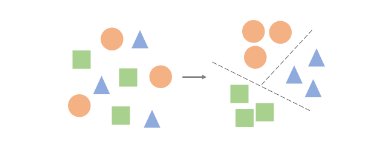
\includegraphics[width=1\textwidth]{imagenes/ml-supervised-learning.png}
    \end{center}
    \caption[Aprendizaje supervisado]{Figura extraída de \cite{sah2020machine} que muestra un ejemplo de aprendizaje supervisado.}
\end{figure}

\subsection{Aprendizaje no supervisado}
Cuando los datos solo vienen en forma de entrada y no se tiene ninguna salida (no hay etiquetas) entonces se trata de un aprendizaje no supervisado. Los algoritmos de este tipo se basan en la diferenciación de los datos mediante los patrones subyacentes que puedan encontrar. Son comunes en el aprendizaje no supervisado los algoritmos de \textit{clustering}~\cite{sah2020machine}.

\begin{figure}[H]
    \begin{center}
        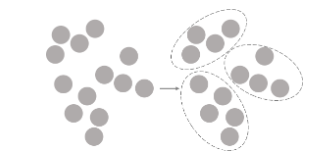
\includegraphics[width=0.7\textwidth]{imagenes/ml_unsupervised-learning.png}
    \end{center}
    \caption[Aprendizaje no supervisado]{Figura extraída de \cite{sah2020machine} que muestra un ejemplo de aprendizaje no supervisado. Se trata de dividir en clústers sin información de etiquetas.}
\end{figure}

\subsection{SVM}
Las máquinas de vectores de soportes o \textit{SVM} fueron introducidas por primera vez en~\cite{cortes_support-vector_1995}. En este documento será uno de los algoritmos de clasificación usados en la función \textit{fitness} para cuantificar la calidad de los pesos aprendidos por los algoritmos optimizadores.\\[6pt]
Las máquinas de vectores de soporte son algoritmos cuya principal característica se basa en la creación de un hiperplano o conjunto de hiperplanos en un espacio $n$-dimensional~\cite{scikit-learn-svm,}. Este hiperplano o hiperplanos es elegido de manera que maximice el margen entre los puntos de datos de todas las clases a predecir. El margen es la distancia entre el hiperplano y los puntos de datos más cercanos de cada clase, estos puntos se denominan vectores de soporte. De esta manera se consigue minimizar el error de generalización~\cite{hastie2009elements}.\\[6pt]
La idea más intuitiva es, que al haber más espacio entre los puntos de distintas clases, hay más posibilidad de que los puntos no vistos, los puntos a predecir, caigan en zonas correctas.

\begin{figure}[H]
    \begin{center}
        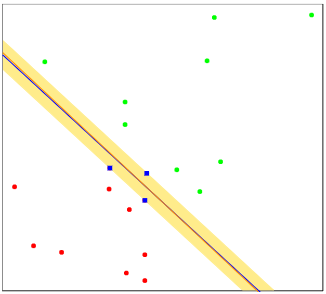
\includegraphics[width=0.5\textwidth]{imagenes/svm-margin.png}
    \end{center}
    \caption[Margen en SVM]{Figura extraída de \cite{hastie2009elements} en la que se muestra de forma gráfica en un espacio $2$-dimensional el margen óptimo de separación de dos clases.}
\end{figure}

\subsection{K-nearest neighbors}
El algoritmo de $k$ vecinos más cercanos fue presentado en \cite{fix_discriminatory_1989} por Evelyn Fix y Joseph Hodges, y más tarde ampliado en \cite{cover_nearest_1967} por Thomas Cover.\\[6pt]
Puede ser utilizado para regresión o clasificación, pero su uso suele darse más en este último problema. Este algoritmo ofrece una premisa sencilla, la clase de un punto $p$ dependerá de cuál sea la clase mayoritaria dentro del subconjunto de $k$ vecinos más cercanos~\cite{10.1007/978-3-540-39964-3_62}.\\[6pt]
Valores mayores de $k$ incrementan la varianza, pero decrementan el sesgo (equilibrio sesgo-varianza~\cite{Mostafa2012}). De forma inversa, a menor $k$ mayor sesgo y menor varianza.\\[6pt]
Otra forma de verlo es que si $k=1$ (el valor mínimo), el modelo entrenado será muy complejo, pues cada punto puede variar de clase por mínimo que sea el cambia en su entorno. Es un modelo que tiende a sobre-ajustar. Con $k=n$ el modelo es lo más simple posible, al tener en cuenta absolutamente todos los puntos, la clasificación será siempre la de la clase más repetida.
\input{capitulos/04_Revisión_de_la_Literatura}
\input{capitulos/05_Descripción_de_los_Algoritmos}
\input{capitulos/06_Diseño_Experimental}
\input{capitulos/07_Análisis_y_Resultados}
%
%\input{capitulos/06_Implementacion}
%
%\input{capitulos/07_Pruebas}
%
%\input{capitulos/06_Conclusiones}
%
%
\nocite{*}
% \bibliography{bibliografia/bibliografia}\addcontentsline{toc}{chapter}{Bibliografía}
% \bibliographystyle{unsrturl}
\newpage
\chapter{Bibliografía}
\printbibliography[heading=none, category=cited]
\appendix
\chapter{}

\begin{figure}[htp]
    \centering
    \includegraphics[width=1\textwidth]{imagenes/fitness_charts/results/real/waveform5000/optimizer_boxplot_fitness_knn_r.png}
    \caption{\textit{Boxplot} waveform5000 - knn - real}

\end{figure}

\begin{figure}[htp]
    \centering
    \includegraphics[width=1\textwidth]{imagenes/fitness_charts/results/real/yeast/optimizer_boxplot_fitness_knn_r.png}
    \caption{\textit{Boxplot} yeast - knn - real}

\end{figure}

\begin{figure}[htp]
    \centering
    \includegraphics[width=1\textwidth]{imagenes/fitness_charts/results/real/spectf-heart/optimizer_boxplot_fitness_knn_r.png}
    \caption{\textit{Boxplot} spectf-heart - knn - real}

\end{figure}

\begin{figure}[htp]
    \centering
    \includegraphics[width=1\textwidth]{imagenes/fitness_charts/results/real/dermatology/optimizer_boxplot_fitness_knn_r.png}
    \caption{\textit{Boxplot} dermatology - knn - real}

\end{figure}

\begin{figure}[htp]
    \centering
    \includegraphics[width=1\textwidth]{imagenes/fitness_charts/results/real/wdbc/optimizer_boxplot_fitness_knn_r.png}
    \caption{\textit{Boxplot} wdbc - knn - real}

\end{figure}

\begin{figure}[htp]
    \centering
    \includegraphics[width=1\textwidth]{imagenes/fitness_charts/results/real/breast-cancer/optimizer_boxplot_fitness_knn_r.png}
    \caption{\textit{Boxplot} breast-cancer - knn - real}

\end{figure}

\begin{figure}[htp]
    \centering
    \includegraphics[width=1\textwidth]{imagenes/fitness_charts/results/real/wine/optimizer_boxplot_fitness_knn_r.png}
    \caption{\textit{Boxplot} wine - knn - real}

\end{figure}

\begin{figure}[htp]
    \centering
    \includegraphics[width=1\textwidth]{imagenes/fitness_charts/results/real/spambase-460/optimizer_boxplot_fitness_knn_r.png}
    \caption{\textit{Boxplot} spambase-460 - knn - real}

\end{figure}

\begin{figure}[htp]
    \centering
    \includegraphics[width=1\textwidth]{imagenes/fitness_charts/results/real/parkinsons/optimizer_boxplot_fitness_knn_r.png}
    \caption{\textit{Boxplot} parkinsons - knn - real}

\end{figure}

\begin{figure}[htp]
    \centering
    \includegraphics[width=1\textwidth]{imagenes/fitness_charts/results/real/sonar/optimizer_boxplot_fitness_knn_r.png}
    \caption{\textit{Boxplot} sonar - knn - real}

\end{figure}

\begin{figure}[htp]
    \centering
    \includegraphics[width=1\textwidth]{imagenes/fitness_charts/results/real/zoo/optimizer_boxplot_fitness_knn_r.png}
    \caption{\textit{Boxplot} zoo - knn - real}

\end{figure}

\begin{figure}[htp]
    \centering
    \includegraphics[width=1\textwidth]{imagenes/fitness_charts/results/real/diabetes/optimizer_boxplot_fitness_knn_r.png}
    \caption{\textit{Boxplot} diabetes - knn - real}

\end{figure}

\begin{figure}[htp]
    \centering
    \includegraphics[width=1\textwidth]{imagenes/fitness_charts/results/real/iris/optimizer_boxplot_fitness_knn_r.png}
    \caption{\textit{Boxplot} iris - knn - real}

\end{figure}

\begin{figure}[htp]
    \centering
    \includegraphics[width=1\textwidth]{imagenes/fitness_charts/results/real/ecoli/optimizer_boxplot_fitness_knn_r.png}
    \caption{\textit{Boxplot} ecoli - knn - real}

\end{figure}

\begin{figure}[htp]
    \centering
    \includegraphics[width=1\textwidth]{imagenes/fitness_charts/results/real/waveform5000/optimizer_boxplot_fitness_svc_r.png}
    \caption{\textit{Boxplot} waveform5000 - svc - real}

\end{figure}

\begin{figure}[htp]
    \centering
    \includegraphics[width=1\textwidth]{imagenes/fitness_charts/results/real/yeast/optimizer_boxplot_fitness_svc_r.png}
    \caption{\textit{Boxplot} yeast - svc - real}

\end{figure}

\begin{figure}[htp]
    \centering
    \includegraphics[width=1\textwidth]{imagenes/fitness_charts/results/real/spectf-heart/optimizer_boxplot_fitness_svc_r.png}
    \caption{\textit{Boxplot} spectf-heart - svc - real}

\end{figure}

\begin{figure}[htp]
    \centering
    \includegraphics[width=1\textwidth]{imagenes/fitness_charts/results/real/dermatology/optimizer_boxplot_fitness_svc_r.png}
    \caption{\textit{Boxplot} dermatology - svc - real}

\end{figure}

\begin{figure}[htp]
    \centering
    \includegraphics[width=1\textwidth]{imagenes/fitness_charts/results/real/wdbc/optimizer_boxplot_fitness_svc_r.png}
    \caption{\textit{Boxplot} wdbc - svc - real}

\end{figure}

\begin{figure}[htp]
    \centering
    \includegraphics[width=1\textwidth]{imagenes/fitness_charts/results/real/breast-cancer/optimizer_boxplot_fitness_svc_r.png}
    \caption{\textit{Boxplot} breast-cancer - svc - real}

\end{figure}

\begin{figure}[htp]
    \centering
    \includegraphics[width=1\textwidth]{imagenes/fitness_charts/results/real/wine/optimizer_boxplot_fitness_svc_r.png}
    \caption{\textit{Boxplot} wine - svc - real}

\end{figure}

\begin{figure}[htp]
    \centering
    \includegraphics[width=1\textwidth]{imagenes/fitness_charts/results/real/spambase-460/optimizer_boxplot_fitness_svc_r.png}
    \caption{\textit{Boxplot} spambase-460 - svc - real}

\end{figure}

\begin{figure}[htp]
    \centering
    \includegraphics[width=1\textwidth]{imagenes/fitness_charts/results/real/parkinsons/optimizer_boxplot_fitness_svc_r.png}
    \caption{\textit{Boxplot} parkinsons - svc - real}

\end{figure}

\begin{figure}[htp]
    \centering
    \includegraphics[width=1\textwidth]{imagenes/fitness_charts/results/real/sonar/optimizer_boxplot_fitness_svc_r.png}
    \caption{\textit{Boxplot} sonar - svc - real}

\end{figure}

\begin{figure}[htp]
    \centering
    \includegraphics[width=1\textwidth]{imagenes/fitness_charts/results/real/zoo/optimizer_boxplot_fitness_svc_r.png}
    \caption{\textit{Boxplot} zoo - svc - real}

\end{figure}

\begin{figure}[htp]
    \centering
    \includegraphics[width=1\textwidth]{imagenes/fitness_charts/results/real/diabetes/optimizer_boxplot_fitness_svc_r.png}
    \caption{\textit{Boxplot} diabetes - svc - real}

\end{figure}

\begin{figure}[htp]
    \centering
    \includegraphics[width=1\textwidth]{imagenes/fitness_charts/results/real/iris/optimizer_boxplot_fitness_svc_r.png}
    \caption{\textit{Boxplot} iris - svc - real}

\end{figure}

\begin{figure}[htp]
    \centering
    \includegraphics[width=1\textwidth]{imagenes/fitness_charts/results/real/ecoli/optimizer_boxplot_fitness_svc_r.png}
    \caption{\textit{Boxplot} ecoli - svc - real}

\end{figure}

\begin{figure}[htp]
    \centering
    \includegraphics[width=1\textwidth]{imagenes/fitness_charts/results/binary/waveform5000/optimizer_boxplot_fitness_knn_b.png}
    \caption{\textit{Boxplot} waveform5000 - knn - binary}

\end{figure}

\begin{figure}[htp]
    \centering
    \includegraphics[width=1\textwidth]{imagenes/fitness_charts/results/binary/yeast/optimizer_boxplot_fitness_knn_b.png}
    \caption{\textit{Boxplot} yeast - knn - binary}

\end{figure}

\begin{figure}[htp]
    \centering
    \includegraphics[width=1\textwidth]{imagenes/fitness_charts/results/binary/spectf-heart/optimizer_boxplot_fitness_knn_b.png}
    \caption{\textit{Boxplot} spectf-heart - knn - binary}

\end{figure}

\begin{figure}[htp]
    \centering
    \includegraphics[width=1\textwidth]{imagenes/fitness_charts/results/binary/dermatology/optimizer_boxplot_fitness_knn_b.png}
    \caption{\textit{Boxplot} dermatology - knn - binary}

\end{figure}

\begin{figure}[htp]
    \centering
    \includegraphics[width=1\textwidth]{imagenes/fitness_charts/results/binary/wdbc/optimizer_boxplot_fitness_knn_b.png}
    \caption{\textit{Boxplot} wdbc - knn - binary}

\end{figure}

\begin{figure}[htp]
    \centering
    \includegraphics[width=1\textwidth]{imagenes/fitness_charts/results/binary/breast-cancer/optimizer_boxplot_fitness_knn_b.png}
    \caption{\textit{Boxplot} breast-cancer - knn - binary}

\end{figure}

\begin{figure}[htp]
    \centering
    \includegraphics[width=1\textwidth]{imagenes/fitness_charts/results/binary/wine/optimizer_boxplot_fitness_knn_b.png}
    \caption{\textit{Boxplot} wine - knn - binary}

\end{figure}

\begin{figure}[htp]
    \centering
    \includegraphics[width=1\textwidth]{imagenes/fitness_charts/results/binary/spambase-460/optimizer_boxplot_fitness_knn_b.png}
    \caption{\textit{Boxplot} spambase-460 - knn - binary}

\end{figure}

\begin{figure}[htp]
    \centering
    \includegraphics[width=1\textwidth]{imagenes/fitness_charts/results/binary/parkinsons/optimizer_boxplot_fitness_knn_b.png}
    \caption{\textit{Boxplot} parkinsons - knn - binary}

\end{figure}

\begin{figure}[htp]
    \centering
    \includegraphics[width=1\textwidth]{imagenes/fitness_charts/results/binary/sonar/optimizer_boxplot_fitness_knn_b.png}
    \caption{\textit{Boxplot} sonar - knn - binary}

\end{figure}

\begin{figure}[htp]
    \centering
    \includegraphics[width=1\textwidth]{imagenes/fitness_charts/results/binary/zoo/optimizer_boxplot_fitness_knn_b.png}
    \caption{\textit{Boxplot} zoo - knn - binary}

\end{figure}

\begin{figure}[htp]
    \centering
    \includegraphics[width=1\textwidth]{imagenes/fitness_charts/results/binary/diabetes/optimizer_boxplot_fitness_knn_b.png}
    \caption{\textit{Boxplot} diabetes - knn - binary}

\end{figure}

\begin{figure}[htp]
    \centering
    \includegraphics[width=1\textwidth]{imagenes/fitness_charts/results/binary/iris/optimizer_boxplot_fitness_knn_b.png}
    \caption{\textit{Boxplot} iris - knn - binary}

\end{figure}

\begin{figure}[htp]
    \centering
    \includegraphics[width=1\textwidth]{imagenes/fitness_charts/results/binary/ecoli/optimizer_boxplot_fitness_knn_b.png}
    \caption{\textit{Boxplot} ecoli - knn - binary}

\end{figure}

\begin{figure}[htp]
    \centering
    \includegraphics[width=1\textwidth]{imagenes/fitness_charts/results/binary/waveform5000/optimizer_boxplot_fitness_svc_b.png}
    \caption{\textit{Boxplot} waveform5000 - svc - binary}

\end{figure}

\begin{figure}[htp]
    \centering
    \includegraphics[width=1\textwidth]{imagenes/fitness_charts/results/binary/yeast/optimizer_boxplot_fitness_svc_b.png}
    \caption{\textit{Boxplot} yeast - svc - binary}

\end{figure}

\begin{figure}[htp]
    \centering
    \includegraphics[width=1\textwidth]{imagenes/fitness_charts/results/binary/spectf-heart/optimizer_boxplot_fitness_svc_b.png}
    \caption{\textit{Boxplot} spectf-heart - svc - binary}

\end{figure}

\begin{figure}[htp]
    \centering
    \includegraphics[width=1\textwidth]{imagenes/fitness_charts/results/binary/dermatology/optimizer_boxplot_fitness_svc_b.png}
    \caption{\textit{Boxplot} dermatology - svc - binary}

\end{figure}

\begin{figure}[htp]
    \centering
    \includegraphics[width=1\textwidth]{imagenes/fitness_charts/results/binary/wdbc/optimizer_boxplot_fitness_svc_b.png}
    \caption{\textit{Boxplot} wdbc - svc - binary}

\end{figure}

\begin{figure}[htp]
    \centering
    \includegraphics[width=1\textwidth]{imagenes/fitness_charts/results/binary/breast-cancer/optimizer_boxplot_fitness_svc_b.png}
    \caption{\textit{Boxplot} breast-cancer - svc - binary}

\end{figure}

\begin{figure}[htp]
    \centering
    \includegraphics[width=1\textwidth]{imagenes/fitness_charts/results/binary/wine/optimizer_boxplot_fitness_svc_b.png}
    \caption{\textit{Boxplot} wine - svc - binary}

\end{figure}

\begin{figure}[htp]
    \centering
    \includegraphics[width=1\textwidth]{imagenes/fitness_charts/results/binary/spambase-460/optimizer_boxplot_fitness_svc_b.png}
    \caption{\textit{Boxplot} spambase-460 - svc - binary}

\end{figure}

\begin{figure}[htp]
    \centering
    \includegraphics[width=1\textwidth]{imagenes/fitness_charts/results/binary/parkinsons/optimizer_boxplot_fitness_svc_b.png}
    \caption{\textit{Boxplot} parkinsons - svc - binary}

\end{figure}

\begin{figure}[htp]
    \centering
    \includegraphics[width=1\textwidth]{imagenes/fitness_charts/results/binary/sonar/optimizer_boxplot_fitness_svc_b.png}
    \caption{\textit{Boxplot} sonar - svc - binary}

\end{figure}

\begin{figure}[htp]
    \centering
    \includegraphics[width=1\textwidth]{imagenes/fitness_charts/results/binary/zoo/optimizer_boxplot_fitness_svc_b.png}
    \caption{\textit{Boxplot} zoo - svc - binary}

\end{figure}

\begin{figure}[htp]
    \centering
    \includegraphics[width=1\textwidth]{imagenes/fitness_charts/results/binary/diabetes/optimizer_boxplot_fitness_svc_b.png}
    \caption{\textit{Boxplot} diabetes - svc - binary}

\end{figure}

\begin{figure}[htp]
    \centering
    \includegraphics[width=1\textwidth]{imagenes/fitness_charts/results/binary/iris/optimizer_boxplot_fitness_svc_b.png}
    \caption{\textit{Boxplot} iris - svc - binary}

\end{figure}

\begin{figure}[htp]
    \centering
    \includegraphics[width=1\textwidth]{imagenes/fitness_charts/results/binary/ecoli/optimizer_boxplot_fitness_svc_b.png}
    \caption{\textit{Boxplot} ecoli - svc - binary}

\end{figure}

\begin{sidewaystable}[htp]
    \centering
    \begin{adjustbox}{width=\linewidth}
        \begin{tabular}{llllllllllllll}
            \toprule
            {}    & abco      & aco       & ba        & cs            & da        & de        & dummy         & fa        & ga        & goa       & gwo           & pso           & woa       \\
            \midrule
            abco  & -         & + (0.083) & + (0.008) & + (0.012)     & + (0.151) & + (0.020) & - (0.018)     & + (0.105) & + (0.012) & + (0.252) & + (0.003)     & + (0.001)     & + (0.012) \\
            aco   & - (0.083) & -         & = (0.514) & = (0.561)     & = (0.679) & = (0.934) & - (0.012)     & + (0.443) & = (0.754) & - (0.389) & + (0.055)     & + (0.081)     & + (0.229) \\
            ba    & - (0.008) & = (0.514) & -         & = (0.851)     & - (0.121) & = (0.900) & - (0.001)     & = (0.890) & = (0.670) & - (0.147) & + (0.055)     & + (0.277)     & = (0.572) \\
            cs    & - (0.012) & = (0.561) & = (0.851) & -             & - (0.320) & = (0.851) & - (1.831E-04) & = (0.679) & = (0.890) & - (0.147) & + (0.135)     & + (0.191)     & = (0.802) \\
            da    & - (0.151) & = (0.679) & + (0.121) & + (0.320)     & -         & + (0.334) & - (0.005)     & + (0.359) & + (0.208) & = (0.599) & + (0.005)     & + (0.030)     & + (0.095) \\
            de    & - (0.020) & = (0.934) & = (0.900) & = (0.851)     & - (0.334) & -         & - (0.007)     & = (0.950) & + (0.454) & - (0.229) & + (0.026)     & + (0.055)     & - (0.233) \\
            dummy & + (0.018) & + (0.012) & + (0.001) & + (1.831E-04) & + (0.005) & + (0.007) & -             & + (0.002) & + (0.002) & + (0.012) & + (6.104E-05) & + (6.104E-05) & + (0.001) \\
            fa    & - (0.105) & - (0.443) & = (0.890) & = (0.679)     & - (0.359) & = (0.950) & - (0.002)     & -         & = (0.660) & - (0.330) & + (0.022)     & + (0.135)     & = (0.639) \\
            ga    & - (0.012) & = (0.754) & = (0.670) & = (0.890)     & - (0.208) & - (0.454) & - (0.002)     & = (0.660) & -         & - (0.050) & + (0.038)     & + (0.272)     & - (0.389) \\
            goa   & - (0.252) & + (0.389) & + (0.147) & + (0.147)     & = (0.599) & + (0.229) & - (0.012)     & + (0.330) & + (0.050) & -         & + (0.010)     & + (0.007)     & + (0.022) \\
            gwo   & - (0.003) & - (0.055) & - (0.055) & - (0.135)     & - (0.005) & - (0.026) & - (6.104E-05) & - (0.022) & - (0.038) & - (0.010) & -             & - (0.346)     & - (0.064) \\
            pso   & - (0.001) & - (0.081) & - (0.277) & - (0.191)     & - (0.030) & - (0.055) & - (6.104E-05) & - (0.135) & - (0.272) & - (0.007) & + (0.346)     & -             & = (0.561) \\
            woa   & - (0.012) & - (0.229) & = (0.572) & = (0.802)     & - (0.095) & + (0.233) & - (0.001)     & = (0.639) & + (0.389) & - (0.022) & + (0.064)     & = (0.561)     & -         \\
            \bottomrule
        \end{tabular}
    \end{adjustbox}
    \caption{P-valores en \textit{fitness} - knn - binario}
\end{sidewaystable}

\begin{sidewaystable}[htp]
    \centering
    \begin{adjustbox}{width=\linewidth}
        \begin{tabular}{llllllllllllll}
            \toprule
            {}    & abco      & aco       & ba        & cs        & da        & de        & dummy         & fa        & ga        & goa       & gwo           & pso           & woa       \\
            \midrule
            abco  & -         & + (0.083) & + (0.256) & + (0.005) & + (0.229) & + (0.035) & - (0.135)     & + (0.041) & + (0.012) & = (0.804) & + (0.002)     & + (0.001)     & + (0.038) \\
            aco   & - (0.083) & -         & - (0.303) & = (0.950) & - (0.208) & = (0.679) & - (0.007)     & - (0.359) & = (0.609) & - (0.073) & + (0.490)     & = (0.887)     & = (0.802) \\
            ba    & - (0.256) & + (0.303) & -         & + (0.015) & = (0.777) & + (0.421) & - (0.003)     & + (0.379) & + (0.044) & - (0.222) & + (0.004)     & + (0.007)     & + (0.208) \\
            cs    & - (0.005) & = (0.950) & - (0.015) & -         & - (0.026) & - (0.451) & - (0.003)     & - (0.421) & = (1.000) & - (0.055) & + (0.364)     & = (0.804)     & - (0.451) \\
            da    & - (0.229) & + (0.208) & = (0.777) & + (0.026) & -         & + (0.277) & - (0.008)     & + (0.454) & + (0.048) & - (0.167) & + (0.005)     & + (0.033)     & + (0.208) \\
            de    & - (0.035) & = (0.679) & - (0.421) & + (0.451) & - (0.277) & -         & - (0.003)     & = (0.802) & = (0.599) & - (0.277) & + (0.109)     & + (0.286)     & = (1.000) \\
            dummy & + (0.135) & + (0.007) & + (0.003) & + (0.003) & + (0.008) & + (0.003) & -             & + (0.015) & + (0.002) & + (0.107) & + (3.052E-04) & + (4.272E-04) & + (0.001) \\
            fa    & - (0.041) & + (0.359) & - (0.379) & + (0.421) & - (0.454) & = (0.802) & - (0.015)     & -         & = (0.820) & - (0.188) & + (0.121)     & + (0.252)     & = (0.599) \\
            ga    & - (0.012) & = (0.609) & - (0.044) & -         & - (0.048) & = (0.599) & - (0.002)     & = (0.820) & -         & - (0.073) & + (0.252)     & + (0.451)     & = (0.706) \\
            goa   & = (0.804) & + (0.073) & + (0.222) & + (0.055) & + (0.167) & + (0.277) & - (0.107)     & + (0.188) & + (0.073) & -         & + (0.008)     & + (0.026)     & + (0.055) \\
            gwo   & - (0.002) & - (0.490) & - (0.004) & - (0.364) & - (0.005) & - (0.109) & - (3.052E-04) & - (0.121) & - (0.252) & - (0.008) & -             & = (0.599)     & - (0.073) \\
            pso   & - (0.001) & = (0.887) & - (0.007) & = (0.804) & - (0.033) & - (0.286) & - (4.272E-04) & - (0.252) & - (0.451) & - (0.026) & = (0.599)     & -             & = (0.570) \\
            woa   & - (0.038) & = (0.802) & - (0.208) & + (0.451) & - (0.208) & -         & - (0.001)     & = (0.599) & = (0.706) & - (0.055) & + (0.073)     & = (0.570)     & -         \\
            \bottomrule
        \end{tabular}
    \end{adjustbox}
    \caption{P-valores en \textit{fitness} - svc - binario}
\end{sidewaystable}

\begin{sidewaystable}[htp]
    \begin{adjustbox}{width=\linewidth}
        \begin{tabular}{llllllllllllll}
            \toprule
            {}   & abco  & aco   & ba    & cs    & da    & de    & dummy  & fa    & ga    & goa   & gwo   & pso   & woa   \\
            \midrule
            F01  & 11    & 1     & 4     & 6     & 9     & 8     & 13     & 12    & 3     & 10    & 2     & 7     & 5     \\
            F02  & 8     & 13    & 7     & 9     & 10    & 4.5   & 12     & 4.5   & 3     & 11    & 1     & 2     & 6     \\
            F03  & 12    & 5     & 9     & 6     & 2     & 8     & 13     & 3     & 10    & 7     & 1     & 4     & 11    \\
            F04  & 12    & 7     & 13    & 1     & 4     & 8     & 10     & 6     & 9     & 11    & 3     & 2     & 5     \\
            F05  & 13    & 5     & 7     & 11    & 10    & 8     & 12     & 1     & 3     & 6     & 4     & 9     & 2     \\
            F06  & 9.5   & 5.5   & 1     & 9.5   & 3     & 9.5   & 13     & 2     & 5.5   & 12    & 5.5   & 5.5   & 9.5   \\
            F07  & 5     & 7     & 2     & 4     & 1     & 13    & 10     & 9     & 11    & 3     & 6     & 8     & 12    \\
            F08  & 8     & 2     & 6.5   & 9     & 12    & 1     & 13     & 11    & 4     & 5     & 10    & 3     & 6.5   \\
            F09  & 10    & 9     & 7     & 1     & 12    & 3     & 13     & 8     & 5     & 11    & 2     & 6     & 4     \\
            F10  & 12    & 13    & 9     & 2     & 10    & 1     & 6      & 7     & 5     & 11    & 3     & 4     & 8     \\
            F11  & 11    & 13    & 8     & 7     & 10    & 5     & 12     & 6     & 2     & 4     & 1     & 3     & 9     \\
            F12  & 13    & 8     & 4.5   & 4.5   & 10    & 11.5  & 11.5   & 9     & 1     & 7     & 2     & 3     & 6     \\
            F13  & 12    & 7.5   & 5     & 10    & 6     & 4     & 13     & 3     & 11    & 9     & 2     & 7.5   & 1     \\
            F14  & 5     & 6     & 3.5   & 10    & 12    & 3.5   & 8      & 8     & 8     & 13    & 2     & 1     & 11    \\
            F15  & 6     & 5     & 9     & 2     & 8     & 7     & 13     & 12    & 11    & 4     & 10    & 3     & 1     \\
            Mean & 9.833 & 7.133 & 6.367 & 6.133 & 7.933 & 6.333 & 11.500 & 6.767 & 6.100 & 8.267 & 3.633 & 4.533 & 6.467 \\
            \bottomrule
        \end{tabular}
    \end{adjustbox}
    \caption{Ranking de los algoritmos en \textit{fitness} - knn - binario}
    \label{tab:ranking_fitness_bin_knn}
\end{sidewaystable}

\begin{sidewaystable}[htp]
    \begin{adjustbox}{width=\linewidth}
        \begin{tabular}{llllllllllllll}
            \toprule
            {}   & abco  & aco   & ba    & cs    & da    & de    & dummy  & fa    & ga    & goa   & gwo   & pso   & woa   \\
            \midrule
            F01  & 9     & 1     & 11    & 13    & 2     & 12    & 6      & 3     & 8     & 7     & 10    & 5     & 4     \\
            F02  & 8     & 11    & 6     & 1     & 9     & 10    & 13     & 2     & 4     & 12    & 7     & 3     & 5     \\
            F03  & 10    & 6     & 8     & 5     & 7     & 13    & 12     & 9     & 2     & 11    & 4     & 3     & 1     \\
            F04  & 7     & 13    & 3     & 1     & 8.5   & 5     & 12     & 10    & 11    & 8.5   & 4     & 6     & 2     \\
            F05  & 13    & 10    & 8     & 1     & 12    & 4     & 11     & 6     & 2     & 7     & 5     & 3     & 9     \\
            F06  & 2     & 4.5   & 10.5  & 4.5   & 10.5  & 1     & 12     & 7     & 8.5   & 13    & 4.5   & 8.5   & 4.5   \\
            F07  & 12    & 2     & 4     & 1     & 7     & 9     & 6      & 13    & 3     & 5     & 8     & 10    & 11    \\
            F08  & 13    & 1     & 12    & 9.5   & 11    & 3     & 6      & 5     & 9.5   & 8     & 2     & 7     & 4     \\
            F09  & 11    & 2     & 8     & 5     & 10    & 9     & 13     & 6     & 3     & 12    & 1     & 7     & 4     \\
            F10  & 6     & 1     & 11    & 10    & 9     & 3     & 13     & 7     & 8     & 2     & 4     & 5     & 12    \\
            F11  & 12    & 13    & 9.5   & 5     & 8     & 5     & 11     & 9.5   & 1     & 7     & 5     & 3     & 2     \\
            F12  & 13    & 2     & 10    & 11    & 9     & 7.5   & 12     & 7.5   & 4.5   & 3     & 1     & 6     & 4.5   \\
            F13  & 8     & 3     & 5     & 6     & 11    & 1     & 10     & 13    & 7     & 12    & 4     & 2     & 9     \\
            F14  & 11    & 3     & 7     & 6     & 8     & 9     & 13     & 4     & 5     & 12    & 2     & 1     & 10    \\
            F15  & 5     & 13    & 10    & 2     & 8     & 6.5   & 12     & 1     & 4     & 11    & 3     & 6.5   & 9     \\
            Mean & 9.333 & 5.700 & 8.200 & 5.400 & 8.667 & 6.533 & 10.800 & 6.867 & 5.367 & 8.700 & 4.300 & 5.067 & 6.067 \\
            \bottomrule
        \end{tabular}
    \end{adjustbox}
    \caption{Ranking de los algoritmos en \textit{fitness} - svc - binario}
    \label{tab:ranking_fitness_bin_svc}
\end{sidewaystable}

\begin{sidewaystable}[htp]
    \begin{adjustbox}{width=\linewidth}
        \begin{tabular}{llllllllllllll}
            \toprule
            {}   & abco      & aco       & ba        & cs        & da        & de        & dummy     & fa        & ga        & goa       & gwo       & pso       & woa       \\
            \midrule
            F01  & 3.640e-01 & 2.350e-01 & 2.960e-01 & 3.320e-01 & 3.560e-01 & 3.540e-01 & 4.330e-01 & 4.210e-01 & 2.640e-01 & 3.570e-01 & 2.630e-01 & 3.410e-01 & 3.230e-01 \\
            F02  & 1.760e-01 & 2.880e-01 & 1.590e-01 & 1.900e-01 & 2.000e-01 & 1.460e-01 & 2.340e-01 & 1.460e-01 & 1.250e-01 & 2.160e-01 & 1.010e-01 & 1.210e-01 & 1.580e-01 \\
            F03  & 3.390e-01 & 3.150e-01 & 3.290e-01 & 3.160e-01 & 2.830e-01 & 3.230e-01 & 3.560e-01 & 2.890e-01 & 3.310e-01 & 3.190e-01 & 2.780e-01 & 2.950e-01 & 3.340e-01 \\
            F04  & 3.150e-01 & 2.800e-01 & 3.310e-01 & 1.950e-01 & 2.510e-01 & 2.810e-01 & 3.030e-01 & 2.680e-01 & 2.940e-01 & 3.140e-01 & 2.290e-01 & 2.160e-01 & 2.630e-01 \\
            F05  & 3.110e-01 & 2.340e-01 & 2.490e-01 & 3.080e-01 & 2.710e-01 & 2.510e-01 & 3.100e-01 & 2.020e-01 & 2.240e-01 & 2.390e-01 & 2.270e-01 & 2.600e-01 & 2.170e-01 \\
            F06  & 1.000e-01 & 8.500e-02 & 2.500e-02 & 1.000e-01 & 5.500e-02 & 1.000e-01 & 1.450e-01 & 2.750e-02 & 8.500e-02 & 1.320e-01 & 8.500e-02 & 8.500e-02 & 1.000e-01 \\
            F07  & 2.100e-01 & 2.300e-01 & 1.980e-01 & 2.080e-01 & 1.760e-01 & 3.260e-01 & 2.450e-01 & 2.360e-01 & 2.490e-01 & 2.030e-01 & 2.140e-01 & 2.330e-01 & 2.590e-01 \\
            F08  & 4.210e-01 & 3.750e-01 & 4.050e-01 & 4.280e-01 & 4.620e-01 & 3.700e-01 & 4.760e-01 & 4.530e-01 & 3.820e-01 & 3.900e-01 & 4.410e-01 & 3.780e-01 & 4.050e-01 \\
            F09  & 2.880e-01 & 2.600e-01 & 2.380e-01 & 1.660e-01 & 2.970e-01 & 1.940e-01 & 3.250e-01 & 2.420e-01 & 2.030e-01 & 2.960e-01 & 1.890e-01 & 2.210e-01 & 2.020e-01 \\
            F10  & 3.440e-01 & 3.550e-01 & 3.200e-01 & 2.820e-01 & 3.290e-01 & 2.790e-01 & 3.040e-01 & 3.080e-01 & 3.030e-01 & 3.410e-01 & 2.890e-01 & 2.990e-01 & 3.090e-01 \\
            F11  & 2.720e-01 & 2.850e-01 & 2.440e-01 & 2.420e-01 & 2.640e-01 & 2.340e-01 & 2.810e-01 & 2.390e-01 & 2.090e-01 & 2.290e-01 & 2.060e-01 & 2.110e-01 & 2.480e-01 \\
            F12  & 1.770e-01 & 1.220e-01 & 1.150e-01 & 1.150e-01 & 1.490e-01 & 1.630e-01 & 1.630e-01 & 1.300e-01 & 9.700e-02 & 1.180e-01 & 1.050e-01 & 1.120e-01 & 1.160e-01 \\
            F13  & 2.660e-01 & 2.070e-01 & 1.850e-01 & 2.410e-01 & 1.880e-01 & 1.790e-01 & 3.330e-01 & 1.610e-01 & 2.430e-01 & 2.400e-01 & 1.050e-01 & 2.070e-01 & 1.040e-01 \\
            F14  & 5.070e-01 & 5.110e-01 & 5.040e-01 & 5.240e-01 & 5.460e-01 & 5.040e-01 & 5.130e-01 & 5.130e-01 & 5.130e-01 & 5.600e-01 & 4.920e-01 & 4.560e-01 & 5.260e-01 \\
            F15  & 3.940e-01 & 3.900e-01 & 4.210e-01 & 3.570e-01 & 4.200e-01 & 3.960e-01 & 4.830e-01 & 4.810e-01 & 4.520e-01 & 3.790e-01 & 4.310e-01 & 3.600e-01 & 2.130e-01 \\
            Best & 0         & 1         & 1         & 2         & 1         & 2         & 0         & 1         & 1         & 0         & 3         & 1         & 2         \\
            \bottomrule
        \end{tabular}
    \end{adjustbox}
    \caption{Media de \textit{fitness} de los algoritmos - knn - binario}
    \label{tab:mean_fitness_bin_knn}
\end{sidewaystable}

\begin{sidewaystable}[htp]
    \begin{adjustbox}{width=\linewidth}
        \begin{tabular}{llllllllllllll}
            \toprule
            {}   & abco      & aco       & ba        & cs        & da        & de        & dummy     & fa        & ga        & goa       & gwo       & pso       & woa       \\
            \midrule
            F01  & 3.080e-01 & 1.940e-01 & 3.460e-01 & 3.620e-01 & 2.170e-01 & 3.470e-01 & 2.920e-01 & 2.580e-01 & 3.020e-01 & 2.980e-01 & 3.110e-01 & 2.820e-01 & 2.640e-01 \\
            F02  & 1.760e-01 & 2.040e-01 & 1.620e-01 & 9.010e-02 & 1.840e-01 & 1.910e-01 & 2.700e-01 & 1.210e-01 & 1.450e-01 & 2.190e-01 & 1.730e-01 & 1.300e-01 & 1.610e-01 \\
            F03  & 3.130e-01 & 2.700e-01 & 2.760e-01 & 2.670e-01 & 2.720e-01 & 3.480e-01 & 3.460e-01 & 2.880e-01 & 2.590e-01 & 3.260e-01 & 2.610e-01 & 2.600e-01 & 2.270e-01 \\
            F04  & 2.990e-01 & 3.530e-01 & 2.680e-01 & 2.310e-01 & 3.010e-01 & 2.820e-01 & 3.490e-01 & 3.230e-01 & 3.450e-01 & 3.010e-01 & 2.790e-01 & 2.920e-01 & 2.610e-01 \\
            F05  & 2.120e-01 & 1.710e-01 & 1.640e-01 & 1.340e-01 & 1.870e-01 & 1.400e-01 & 1.740e-01 & 1.570e-01 & 1.360e-01 & 1.610e-01 & 1.460e-01 & 1.380e-01 & 1.680e-01 \\
            F06  & 1.000e-01 & 1.150e-01 & 1.450e-01 & 1.150e-01 & 1.450e-01 & 7.000e-02 & 2.400e-01 & 1.200e-01 & 1.300e-01 & 3.020e-01 & 1.150e-01 & 1.300e-01 & 1.150e-01 \\
            F07  & 2.870e-01 & 2.070e-01 & 2.240e-01 & 2.010e-01 & 2.360e-01 & 2.480e-01 & 2.290e-01 & 3.100e-01 & 2.210e-01 & 2.260e-01 & 2.440e-01 & 2.540e-01 & 2.660e-01 \\
            F08  & 4.530e-01 & 3.330e-01 & 4.470e-01 & 4.260e-01 & 4.440e-01 & 3.620e-01 & 3.880e-01 & 3.860e-01 & 4.260e-01 & 3.990e-01 & 3.340e-01 & 3.890e-01 & 3.680e-01 \\
            F09  & 3.190e-01 & 1.740e-01 & 2.580e-01 & 2.080e-01 & 2.740e-01 & 2.670e-01 & 3.820e-01 & 2.140e-01 & 1.810e-01 & 3.690e-01 & 1.720e-01 & 2.400e-01 & 1.910e-01 \\
            F10  & 2.800e-01 & 2.270e-01 & 3.130e-01 & 2.910e-01 & 2.900e-01 & 2.740e-01 & 3.930e-01 & 2.840e-01 & 2.850e-01 & 2.410e-01 & 2.770e-01 & 2.780e-01 & 3.540e-01 \\
            F11  & 2.370e-01 & 2.480e-01 & 2.040e-01 & 1.920e-01 & 2.020e-01 & 1.920e-01 & 2.350e-01 & 2.040e-01 & 1.800e-01 & 2.000e-01 & 1.920e-01 & 1.870e-01 & 1.840e-01 \\
            F12  & 1.600e-01 & 8.780e-02 & 1.350e-01 & 1.440e-01 & 1.320e-01 & 1.310e-01 & 1.520e-01 & 1.310e-01 & 1.110e-01 & 8.800e-02 & 5.510e-02 & 1.150e-01 & 1.110e-01 \\
            F13  & 3.230e-01 & 2.200e-01 & 2.700e-01 & 2.960e-01 & 3.770e-01 & 2.050e-01 & 3.380e-01 & 4.100e-01 & 3.040e-01 & 4.060e-01 & 2.640e-01 & 2.140e-01 & 3.330e-01 \\
            F14  & 5.250e-01 & 4.910e-01 & 5.080e-01 & 5.000e-01 & 5.110e-01 & 5.210e-01 & 5.750e-01 & 4.980e-01 & 4.990e-01 & 5.410e-01 & 4.800e-01 & 4.590e-01 & 5.220e-01 \\
            F15  & 3.210e-01 & 5.690e-01 & 3.840e-01 & 3.010e-01 & 3.360e-01 & 3.240e-01 & 4.860e-01 & 2.460e-01 & 3.070e-01 & 4.340e-01 & 3.040e-01 & 3.240e-01 & 3.550e-01 \\
            Best & 0         & 3         & 0         & 4         & 0         & 2         & 0         & 1         & 1         & 0         & 2         & 1         & 1         \\
            \bottomrule
        \end{tabular}
    \end{adjustbox}
    \caption{Media de \textit{fitness} de los algoritmos - svc - binario}
    \label{tab:mean_fitness_bin_svc}
\end{sidewaystable}

\begin{sidewaystable}[htp]
    \centering
    \begin{adjustbox}{width=\linewidth}
        \begin{tabular}{llllllllllllll}
            \toprule
            {}    & abco      & aco       & ba        & cs        & da        & de        & dummy     & fa        & ga        & goa       & gwo       & pso       & woa       \\
            \midrule
            abco  & -         & - (0.015) & + (0.402) & = (0.784) & - (0.346) & = (0.529) & - (0.008) & = (0.679) & = (0.649) & - (0.379) & + (0.414) & + (0.196) & + (0.410) \\
            aco   & + (0.015) & -         & + (0.003) & + (0.038) & + (0.045) & + (0.038) & + (0.451) & + (0.026) & + (0.081) & + (0.021) & + (0.012) & + (0.014) & + (0.004) \\
            ba    & - (0.402) & - (0.003) & -         & - (0.307) & - (0.069) & = (0.875) & - (0.010) & = (0.802) & - (0.061) & - (0.038) & = (0.802) & = (0.616) & = (0.950) \\
            cs    & = (0.784) & - (0.038) & + (0.307) & -         & - (0.451) & = (0.944) & - (0.045) & = (0.934) & = (0.551) & = (0.762) & = (0.762) & = (0.720) & = (0.576) \\
            da    & + (0.346) & - (0.045) & + (0.069) & + (0.451) & -         & + (0.346) & - (0.233) & + (0.191) & = (0.934) & = (0.934) & + (0.121) & + (0.132) & + (0.117) \\
            de    & = (0.529) & - (0.038) & = (0.875) & = (0.944) & - (0.346) & -         & - (0.059) & = (0.762) & - (0.346) & - (0.421) & + (0.389) & = (0.720) & + (0.315) \\
            dummy & + (0.008) & - (0.451) & + (0.010) & + (0.045) & + (0.233) & + (0.059) & -         & + (0.060) & + (0.252) & + (0.155) & + (0.028) & + (0.008) & + (0.048) \\
            fa    & = (0.679) & - (0.026) & = (0.802) & = (0.934) & - (0.191) & = (0.762) & - (0.060) & -         & - (0.167) & - (0.330) & = (0.802) & = (0.950) & = (0.932) \\
            ga    & = (0.649) & - (0.081) & + (0.061) & = (0.551) & = (0.934) & + (0.346) & - (0.252) & + (0.167) & -         & = (0.906) & + (0.081) & + (0.162) & + (0.263) \\
            goa   & + (0.379) & - (0.021) & + (0.038) & = (0.762) & = (0.934) & + (0.421) & - (0.155) & + (0.330) & = (0.906) & -         & + (0.233) & + (0.196) & + (0.107) \\
            gwo   & - (0.414) & - (0.012) & = (0.802) & = (0.762) & - (0.121) & - (0.389) & - (0.028) & = (0.802) & - (0.081) & - (0.233) & -         & = (0.572) & = (0.802) \\
            pso   & - (0.196) & - (0.014) & = (0.616) & = (0.720) & - (0.132) & = (0.720) & - (0.008) & = (0.950) & - (0.162) & - (0.196) & = (0.572) & -         & = (0.934) \\
            woa   & - (0.410) & - (0.004) & = (0.950) & = (0.576) & - (0.117) & - (0.315) & - (0.048) & = (0.932) & - (0.263) & - (0.107) & = (0.802) & = (0.934) & -         \\
            \bottomrule
        \end{tabular}
    \end{adjustbox}
    \caption{P-valores en \textit{accuracy} - knn - binario}
    \label{tab:p-values_accuracy_bin_knn}
\end{sidewaystable}

\begin{sidewaystable}[htp]
    \centering
    \begin{adjustbox}{width=\linewidth}
        \begin{tabular}{llllllllllllll}
            \toprule
            {}    & abco      & aco       & ba        & cs        & da        & de        & dummy     & fa        & ga        & goa       & gwo       & pso       & woa       \\
            \midrule
            abco  & -         & - (0.209) & = (0.660) & + (0.463) & - (0.083) & = (0.890) & - (0.064) & = (0.720) & - (0.156) & - (0.095) & = (0.890) & = (0.934) & = (1.000) \\
            aco   & + (0.209) & -         & + (0.330) & + (0.167) & = (0.530) & + (0.116) & = (0.934) & + (0.117) & + (0.359) & = (0.720) & + (0.079) & + (0.188) & + (0.124) \\
            ba    & = (0.660) & - (0.330) & -         & + (0.094) & - (0.162) & + (0.490) & - (0.151) & + (0.389) & = (0.689) & - (0.167) & + (0.421) & + (0.286) & = (0.551) \\
            cs    & - (0.463) & - (0.167) & - (0.094) & -         & - (0.026) & = (0.706) & - (0.064) & = (0.826) & - (0.055) & - (0.095) & = (0.706) & = (0.510) & - (0.490) \\
            da    & + (0.083) & = (0.530) & + (0.162) & + (0.026) & -         & + (0.196) & - (0.330) & + (0.121) & + (0.327) & - (0.359) & + (0.149) & + (0.132) & + (0.208) \\
            de    & = (0.890) & - (0.116) & - (0.490) & = (0.706) & - (0.196) & -         & - (0.060) & = (0.660) & - (0.402) & - (0.229) & -         & = (0.720) & = (0.847) \\
            dummy & + (0.064) & = (0.934) & + (0.151) & + (0.064) & + (0.330) & + (0.060) & -         & + (0.142) & + (0.303) & = (0.890) & + (0.055) & + (0.048) & + (0.055) \\
            fa    & = (0.720) & - (0.117) & - (0.389) & = (0.826) & - (0.121) & = (0.660) & - (0.142) & -         & - (0.182) & - (0.209) & = (0.784) & - (0.470) & = (0.950) \\
            ga    & + (0.156) & - (0.359) & = (0.689) & + (0.055) & - (0.327) & + (0.402) & - (0.303) & + (0.182) & -         & - (0.454) & + (0.233) & + (0.290) & = (0.514) \\
            goa   & + (0.095) & = (0.720) & + (0.167) & + (0.095) & + (0.359) & + (0.229) & = (0.890) & + (0.209) & + (0.454) & -         & + (0.117) & + (0.135) & + (0.083) \\
            gwo   & = (0.890) & - (0.079) & - (0.421) & = (0.706) & - (0.149) & = (1.000) & - (0.055) & = (0.784) & - (0.233) & - (0.117) & -         & = (0.660) & = (0.727) \\
            pso   & = (0.934) & - (0.188) & - (0.286) & = (0.510) & - (0.132) & = (0.720) & - (0.048) & + (0.470) & - (0.290) & - (0.135) & = (0.660) & -         & = (0.802) \\
            woa   & -         & - (0.124) & = (0.551) & + (0.490) & - (0.208) & = (0.847) & - (0.055) & = (0.950) & = (0.514) & - (0.083) & = (0.727) & = (0.802) & -         \\
            \bottomrule
        \end{tabular}
    \end{adjustbox}
    \caption{P-valores en \textit{accuracy} - svc - binario}
    \label{tab:p-values_accuracy_bin_svc}
\end{sidewaystable}

\begin{sidewaystable}[htp]
    \centering
    \begin{adjustbox}{width=\linewidth}
        \begin{tabular}{llllllllllllll}
            \toprule
            {}   & abco  & aco    & ba    & cs    & da    & de    & dummy & fa    & ga    & goa   & gwo   & pso   & woa   \\
            \midrule
            F01  & 5.5   & 1      & 4     & 7     & 11    & 9     & 12    & 13    & 2.5   & 8     & 2.5   & 10    & 5.5   \\
            F02  & 6.5   & 13     & 6.5   & 9.5   & 9.5   & 4.5   & 11    & 2.5   & 4.5   & 12    & 1     & 2.5   & 8     \\
            F03  & 7     & 12     & 9     & 7     & 2     & 7     & 10    & 1     & 13    & 4     & 3     & 5     & 11    \\
            F04  & 9     & 12     & 13    & 1     & 4.5   & 7.5   & 7.5   & 6     & 10.5  & 10.5  & 3     & 2     & 4.5   \\
            F05  & 9     & 11.5   & 3     & 13    & 9     & 6     & 11.5  & 1     & 4.5   & 4.5   & 7     & 9     & 2     \\
            F06  & 10.5  & 6      & 1.5   & 10.5  & 3     & 10.5  & 13    & 1.5   & 6     & 6     & 6     & 6     & 10.5  \\
            F07  & 2     & 11.5   & 3     & 5.5   & 1     & 13    & 5.5   & 7     & 11.5  & 4     & 8     & 9     & 10    \\
            F08  & 2.5   & 8.5    & 4.5   & 8.5   & 13    & 1     & 10.5  & 10.5  & 6.5   & 4.5   & 12    & 2.5   & 6.5   \\
            F09  & 9     & 13     & 6.5   & 1     & 10.5  & 2     & 10.5  & 8     & 5     & 12    & 4     & 6.5   & 3     \\
            F10  & 6.5   & 13     & 6.5   & 3     & 11    & 1.5   & 1.5   & 4     & 10    & 12    & 6.5   & 9     & 6.5   \\
            F11  & 8     & 13     & 7     & 10    & 12    & 5     & 11    & 3.5   & 1.5   & 6     & 3.5   & 1.5   & 9     \\
            F12  & 10    & 12.5   & 1     & 3     & 11    & 12.5  & 8.5   & 5.5   & 3     & 5.5   & 8.5   & 7     & 3     \\
            F13  & 10.5  & 8      & 5     & 10.5  & 5     & 5     & 13    & 3     & 12    & 8     & 2     & 8     & 1     \\
            F14  & 3     & 11     & 4     & 10    & 13    & 6     & 2     & 7     & 9     & 12    & 5     & 1     & 8     \\
            F15  & 4     & 8      & 8     & 2     & 8     & 6     & 10.5  & 12.5  & 12.5  & 4     & 10.5  & 4     & 1     \\
            Mean & 6.867 & 10.267 & 5.500 & 6.767 & 8.233 & 6.433 & 9.200 & 5.733 & 7.467 & 7.533 & 5.500 & 5.533 & 5.967 \\
            \bottomrule
        \end{tabular}
    \end{adjustbox}
    \caption{Ranking de los algoritmos en \textit{accuracy} - knn - binario}
    \label{tab:ranking_accuracy_bin_knn}
\end{sidewaystable}

\begin{sidewaystable}[htp]
    \centering
    \begin{adjustbox}{width=\linewidth}
        \begin{tabular}{llllllllllllll}
            \toprule
            {}   & abco  & aco   & ba    & cs    & da    & de    & dummy & fa    & ga    & goa   & gwo   & pso   & woa   \\
            \midrule
            F01  & 6     & 1.5   & 11.5  & 13    & 1.5   & 11.5  & 3.5   & 3.5   & 9     & 7     & 10    & 8     & 5     \\
            F02  & 4.5   & 13    & 4.5   & 1     & 8     & 9     & 12    & 2     & 7     & 11    & 10    & 3     & 6     \\
            F03  & 9     & 10    & 4.5   & 2     & 6     & 13    & 12    & 7.5   & 4.5   & 11    & 7.5   & 3     & 1     \\
            F04  & 4     & 13    & 2.5   & 1     & 9     & 5     & 11    & 10    & 12    & 6     & 7     & 8     & 2.5   \\
            F05  & 11    & 13    & 6     & 1.5   & 12    & 1.5   & 3     & 4     & 6     & 8.5   & 8.5   & 6     & 10    \\
            F06  & 2     & 5     & 10.5  & 5     & 10.5  & 1     & 12    & 5     & 8.5   & 13    & 5     & 8.5   & 5     \\
            F07  & 8.5   & 8.5   & 3.5   & 2     & 6     & 6     & 1     & 13    & 6     & 3.5   & 11    & 11    & 11    \\
            F08  & 9     & 6     & 11    & 10    & 12.5  & 2.5   & 2.5   & 5     & 12.5  & 8     & 1     & 7     & 4     \\
            F09  & 11    & 6     & 7     & 5     & 10    & 9     & 12    & 4     & 3     & 13    & 1     & 8     & 2     \\
            F10  & 1     & 6     & 10.5  & 7.5   & 9     & 4     & 13    & 4     & 10.5  & 2     & 4     & 7.5   & 12    \\
            F11  & 8     & 13    & 4.5   & 2     & 9     & 3     & 11    & 6.5   & 4.5   & 10    & 12    & 6.5   & 1     \\
            F12  & 4     & 7.5   & 9.5   & 13    & 9.5   & 7.5   & 5.5   & 5.5   & 11.5  & 2     & 1     & 11.5  & 3     \\
            F13  & 6.5   & 3     & 4     & 6.5   & 11    & 1     & 8     & 12.5  & 9     & 12.5  & 5     & 2     & 10    \\
            F14  & 7     & 12    & 4     & 5.5   & 8.5   & 8.5   & 13    & 3     & 5.5   & 11    & 2     & 1     & 10    \\
            F15  & 2.5   & 13    & 10    & 2.5   & 5.5   & 5.5   & 12    & 1     & 5.5   & 11    & 5.5   & 8     & 9     \\
            Mean & 6.267 & 8.700 & 6.900 & 5.167 & 8.533 & 5.867 & 8.767 & 5.767 & 7.667 & 8.633 & 6.033 & 6.600 & 6.100 \\
            \bottomrule
        \end{tabular}
    \end{adjustbox}
    \caption{Ranking de los algoritmos en \textit{accuracy} - svc - binario}
    \label{tab:ranking_accuracy_bin_svc}
\end{sidewaystable}

\begin{sidewaystable}[htp]
    \centering
    \begin{adjustbox}{width=\linewidth}
        \begin{tabular}{llllllllllllll}
            \toprule
            {}    & abco          & aco           & ba            & cs            & da        & de            & dummy         & fa            & ga            & goa           & gwo           & pso           & woa           \\
            \midrule
            abco  & -             & + (0.001)     & + (0.001)     & + (0.001)     & + (0.001) & + (0.001)     & = (0.820)     & + (1.831E-04) & + (0.001)     & + (0.015)     & + (0.001)     & + (0.001)     & + (0.001)     \\
            aco   & - (0.001)     & -             & - (0.001)     & - (0.001)     & - (0.001) & - (0.001)     & - (6.104E-05) & - (6.104E-05) & - (0.001)     & - (6.104E-05) & - (0.002)     & - (0.001)     & - (0.001)     \\
            ba    & - (0.001)     & + (0.001)     & -             & + (0.001)     & + (0.014) & + (0.010)     & - (6.104E-05) & = (0.570)     & + (0.001)     & = (0.934)     & + (0.001)     & + (0.001)     & + (0.002)     \\
            cs    & - (0.001)     & + (0.001)     & - (0.001)     & -             & - (0.149) & - (0.001)     & - (6.104E-05) & - (0.001)     & + (0.001)     & - (0.029)     & + (0.001)     & + (0.001)     & - (0.208)     \\
            da    & - (0.001)     & + (0.001)     & - (0.014)     & + (0.149)     & -         & = (0.778)     & - (0.001)     & - (0.005)     & + (0.001)     & = (0.524)     & + (0.001)     & + (0.002)     & + (0.485)     \\
            de    & - (0.001)     & + (0.001)     & - (0.010)     & + (0.001)     & = (0.778) & -             & - (6.104E-05) & - (1.831E-04) & + (0.001)     & - (0.359)     & + (0.001)     & + (0.001)     & + (0.117)     \\
            dummy & = (0.820)     & + (6.104E-05) & + (6.104E-05) & + (6.104E-05) & + (0.001) & + (6.104E-05) & -             & + (0.001)     & + (6.104E-05) & + (0.001)     & + (6.104E-05) & + (6.104E-05) & + (6.104E-05) \\
            fa    & - (1.831E-04) & + (6.104E-05) & = (0.570)     & + (0.001)     & + (0.005) & + (1.831E-04) & - (0.001)     & -             & + (6.104E-05) & + (0.258)     & + (6.104E-05) & + (6.104E-05) & + (0.002)     \\
            ga    & - (0.001)     & + (0.001)     & - (0.001)     & - (0.001)     & - (0.001) & - (0.001)     & - (6.104E-05) & - (6.104E-05) & -             & - (6.104E-05) & + (0.031)     & - (0.013)     & - (0.001)     \\
            goa   & - (0.015)     & + (6.104E-05) & = (0.934)     & + (0.029)     & = (0.524) & + (0.359)     & - (0.001)     & - (0.258)     & + (6.104E-05) & -             & + (6.104E-05) & + (0.001)     & + (0.201)     \\
            gwo   & - (0.001)     & + (0.002)     & - (0.001)     & - (0.001)     & - (0.001) & - (0.001)     & - (6.104E-05) & - (6.104E-05) & - (0.031)     & - (6.104E-05) & -             & - (0.002)     & - (0.001)     \\
            pso   & - (0.001)     & + (0.001)     & - (0.001)     & - (0.001)     & - (0.002) & - (0.001)     & - (6.104E-05) & - (6.104E-05) & + (0.013)     & - (0.001)     & + (0.002)     & -             & - (0.001)     \\
            woa   & - (0.001)     & + (0.001)     & - (0.002)     & + (0.208)     & - (0.485) & - (0.117)     & - (6.104E-05) & - (0.002)     & + (0.001)     & - (0.201)     & + (0.001)     & + (0.001)     & -             \\
            \bottomrule
        \end{tabular}
    \end{adjustbox}
    \caption{P-valores en ratio de selección - knn - binario}
    \label{tab:p-values_sel_ratio_bin_knn}
\end{sidewaystable}

\begin{sidewaystable}[htp]
    \centering
    \begin{adjustbox}{width=\linewidth}
        \begin{tabular}{llllllllllllll}
            \toprule
            {}    & abco          & aco           & ba            & cs            & da            & de            & dummy         & fa            & ga            & goa           & gwo           & pso           & woa       \\
            \midrule
            abco  & -             & + (0.001)     & + (0.001)     & + (0.001)     & + (0.001)     & + (0.001)     & = (0.847)     & + (1.831E-04) & + (0.001)     & + (0.010)     & + (0.001)     & + (0.001)     & + (0.001) \\
            aco   & - (0.001)     & -             & - (0.001)     & - (0.001)     & - (0.001)     & - (0.001)     & - (6.104E-05) & - (6.104E-05) & - (0.001)     & - (6.104E-05) & - (0.001)     & - (0.001)     & - (0.001) \\
            ba    & - (0.001)     & + (0.001)     & -             & + (0.001)     & + (0.003)     & + (0.017)     & - (6.104E-05) & - (0.489)     & + (0.001)     & = (0.804)     & + (0.001)     & + (0.001)     & + (0.001) \\
            cs    & - (0.001)     & + (0.001)     & - (0.001)     & -             & = (0.851)     & - (0.004)     & - (6.104E-05) & - (6.104E-05) & + (0.001)     & - (0.033)     & + (0.001)     & + (0.001)     & - (0.279) \\
            da    & - (0.001)     & + (0.001)     & - (0.003)     & = (0.851)     & -             & - (0.090)     & - (6.104E-05) & - (6.104E-05) & + (0.002)     & - (0.244)     & + (0.004)     & + (0.001)     & = (0.706) \\
            de    & - (0.001)     & + (0.001)     & - (0.017)     & + (0.004)     & + (0.090)     & -             & - (6.104E-05) & - (0.004)     & + (0.001)     & - (0.330)     & + (0.001)     & + (0.001)     & + (0.015) \\
            dummy & = (0.847)     & + (6.104E-05) & + (6.104E-05) & + (6.104E-05) & + (6.104E-05) & + (6.104E-05) & -             & + (6.104E-05) & + (6.104E-05) & + (0.001)     & + (6.104E-05) & + (6.104E-05) & + (0.001) \\
            fa    & - (1.831E-04) & + (6.104E-05) & + (0.489)     & + (6.104E-05) & + (6.104E-05) & + (0.004)     & - (6.104E-05) & -             & + (6.104E-05) & = (0.890)     & + (6.104E-05) & + (0.001)     & + (0.001) \\
            ga    & - (0.001)     & + (0.001)     & - (0.001)     & - (0.001)     & - (0.002)     & - (0.001)     & - (6.104E-05) & - (6.104E-05) & -             & - (6.104E-05) & + (0.233)     & - (0.055)     & - (0.001) \\
            goa   & - (0.010)     & + (6.104E-05) & = (0.804)     & + (0.033)     & + (0.244)     & + (0.330)     & - (0.001)     & = (0.890)     & + (6.104E-05) & -             & + (3.052E-04) & + (6.104E-05) & + (0.083) \\
            gwo   & - (0.001)     & + (0.001)     & - (0.001)     & - (0.001)     & - (0.004)     & - (0.001)     & - (6.104E-05) & - (6.104E-05) & - (0.233)     & - (3.052E-04) & -             & - (0.184)     & - (0.002) \\
            pso   & - (0.001)     & + (0.001)     & - (0.001)     & - (0.001)     & - (0.001)     & - (0.001)     & - (6.104E-05) & - (0.001)     & + (0.055)     & - (6.104E-05) & + (0.184)     & -             & - (0.001) \\
            woa   & - (0.001)     & + (0.001)     & - (0.001)     & + (0.279)     & = (0.706)     & - (0.015)     & - (0.001)     & - (0.001)     & + (0.001)     & - (0.083)     & + (0.002)     & + (0.001)     & -         \\
            \bottomrule
        \end{tabular}
    \end{adjustbox}
    \caption{P-valores en ratio de selección - svc - binario}
    \label{tab:p-values_sel_ratio_bin_svc}
\end{sidewaystable}

\begin{sidewaystable}[htp]
    \centering
    \begin{adjustbox}{width=\linewidth}
        \begin{tabular}{llllllllllllll}
            \toprule
            {}   & abco   & aco   & ba    & cs    & da    & de    & dummy  & fa    & ga    & goa   & gwo   & pso   & woa   \\
            \midrule
            F01  & 13     & 1     & 8     & 7     & 4.5   & 9     & 12     & 10    & 3     & 11    & 2     & 4.5   & 6     \\
            F02  & 12     & 1     & 11    & 6     & 9     & 8     & 13     & 10    & 3     & 7     & 2     & 4     & 5     \\
            F03  & 12     & 1     & 8     & 7     & 6     & 9     & 13     & 10    & 2.5   & 11    & 2.5   & 4     & 5     \\
            F04  & 13     & 1     & 10    & 6     & 5     & 7     & 12     & 8     & 3     & 11    & 3     & 3     & 9     \\
            F05  & 13     & 1     & 11    & 8     & 6     & 9     & 12     & 10    & 3     & 5     & 2     & 4     & 7     \\
            F06  & 5.5    & 5.5   & 5.5   & 5.5   & 5.5   & 5.5   & 12     & 11    & 5.5   & 13    & 5.5   & 5.5   & 5.5   \\
            F07  & 12     & 1     & 9     & 5     & 10    & 6     & 13     & 11    & 3     & 8     & 2     & 4     & 7     \\
            F08  & 13     & 1     & 11    & 8     & 6     & 9     & 12     & 10    & 2     & 5     & 3     & 4     & 7     \\
            F09  & 13     & 1     & 11    & 6     & 8     & 9     & 12     & 10    & 2     & 5     & 3     & 4     & 7     \\
            F10  & 13     & 1     & 11    & 5     & 7     & 9     & 12     & 10    & 3     & 6     & 2     & 4     & 8     \\
            F11  & 13     & 1     & 10    & 5     & 9     & 8     & 12     & 11    & 3     & 6     & 2     & 4     & 7     \\
            F12  & 13     & 1     & 11    & 6     & 8     & 9     & 12     & 10    & 3     & 5     & 2     & 4     & 7     \\
            F13  & 12     & 1.5   & 8     & 5     & 9     & 6     & 13     & 10.5  & 4     & 10.5  & 1.5   & 3     & 7     \\
            F14  & 11     & 1     & 8     & 7     & 9.5   & 6     & 12     & 5     & 3.5   & 13    & 2     & 3.5   & 9.5   \\
            F15  & 12     & 1     & 10    & 5.5   & 9     & 7     & 13     & 11    & 4     & 8     & 2     & 3     & 5.5   \\
            Mean & 12.033 & 1.333 & 9.500 & 6.133 & 7.433 & 7.767 & 12.333 & 9.833 & 3.167 & 8.300 & 2.433 & 3.900 & 6.833 \\
            \bottomrule
        \end{tabular}
    \end{adjustbox}
    \caption{Ranking de los algoritmos en seleccion de caracteristicas - knn - binario}
    \label{tab:ranking_sel_rate_bin_knn}
\end{sidewaystable}

\begin{sidewaystable}[htp]
    \centering
    \begin{adjustbox}{width=\linewidth}
        \begin{tabular}{llllllllllllll}
            \toprule
            {}   & abco   & aco   & ba    & cs    & da    & de    & dummy  & fa     & ga    & goa   & gwo   & pso   & woa   \\
            \midrule
            F01  & 12     & 1     & 7     & 6     & 5     & 8.5   & 13     & 10     & 2     & 11    & 3     & 4     & 8.5   \\
            F02  & 12     & 1     & 10    & 5     & 9     & 6.5   & 13     & 11     & 3     & 8     & 2     & 4     & 6.5   \\
            F03  & 12     & 1     & 8     & 7     & 6     & 9     & 13     & 10     & 3     & 11    & 2     & 4     & 5     \\
            F04  & 13     & 1     & 9     & 7     & 5     & 10    & 11     & 8      & 4     & 12    & 2.5   & 2.5   & 6     \\
            F05  & 13     & 1     & 11    & 7     & 8     & 9     & 12     & 10     & 3     & 5     & 2     & 4     & 6     \\
            F06  & 5.5    & 5.5   & 5.5   & 5.5   & 5.5   & 5.5   & 12     & 11     & 5.5   & 13    & 5.5   & 5.5   & 5.5   \\
            F07  & 13     & 1     & 8     & 5     & 6     & 9     & 12     & 11     & 2     & 10    & 3     & 4     & 7     \\
            F08  & 13     & 1     & 11    & 7     & 5     & 9     & 12     & 10     & 2     & 4     & 6     & 3     & 8     \\
            F09  & 13     & 1     & 11    & 6     & 9     & 8     & 12     & 10     & 2     & 5     & 3     & 4     & 7     \\
            F10  & 13     & 1     & 11    & 9     & 5     & 6     & 12     & 10     & 2     & 4     & 7.5   & 3     & 7.5   \\
            F11  & 13     & 1     & 11    & 9     & 6     & 8     & 12     & 10     & 3.5   & 5     & 2     & 3.5   & 7     \\
            F12  & 13     & 1     & 10    & 5     & 8     & 9     & 12     & 11     & 3     & 7     & 2     & 4     & 6     \\
            F13  & 12     & 2     & 9     & 6     & 7     & 5     & 13     & 11     & 3.5   & 10    & 1     & 3.5   & 8     \\
            F14  & 11     & 1     & 10    & 6     & 4     & 9     & 12     & 7.5    & 5     & 13    & 3     & 2     & 7.5   \\
            F15  & 12     & 1     & 9     & 5.5   & 10    & 7     & 13     & 11     & 4     & 8     & 2     & 3     & 5.5   \\
            Mean & 12.033 & 1.367 & 9.367 & 6.400 & 6.567 & 7.900 & 12.267 & 10.100 & 3.167 & 8.400 & 3.100 & 3.600 & 6.733 \\
            \bottomrule
        \end{tabular}
    \end{adjustbox}
    \caption{Ranking de los algoritmos en seleccion de caracteristicas - svc - binario}
    \label{tab:ranking_sel_rate_bin_svc}
\end{sidewaystable}

\begin{sidewaystable}[htp]
    \centering
    \begin{adjustbox}{width=\linewidth}
        \begin{tabular}{lllllllllllllllll}
            \toprule
                      &                          & dataset       &             &          &         &            &         &            &         &              &              &              &         &         &         & \tabularnewline
            optimizer & Data                     & breast-cancer & dermatology & diabetes & ecoli   & ionosphere & iris    & parkinsons & sonar   & spambase-460 & spectf-heart & waveform5000 & wdbc    & wine    & yeast   & zoo\tabularnewline
            \midrule
            abco      & Average - acc            & 74.17\%       & 88.00\%     & 73.23\%  & 77.14\% & 85.33\%    & 91.67\% & 77.50\%    & 60.00\% & 74.74\%      & 79.29\%      & 83.75\%      & 91.74\% & 71.25\% & 51.33\% & 70.00\%\tabularnewline
                      & Average - selected\_rate & 75.56\%       & 67.65\%     & 72.50\%  & 92.86\% & 80.00\%    & 25.00\% & 84.55\%    & 92.67\% & 91.58\%      & 93.64\%      & 91.00\%      & 85.33\% & 63.85\% & 87.50\% & 51.18\%\tabularnewline
            aco       & Average - acc            & 79.17\%       & 78.67\%     & 71.94\%  & 65.71\% & 82.00\%    & 90.00\% & 77.50\%    & 63.33\% & 81.05\%      & 75.00\%      & 73.45\%      & 90.87\% & 77.50\% & 50.00\% & 38.00\%\tabularnewline
                      & Average - selected\_rate & 6.67\%        & 12.35\%     & 17.50\%  & 44.29\% & 8.53\%     & 25.00\% & 4.09\%     & 2.50\%  & 3.33\%       & 1.82\%       & 9.25\%       & 5.67\%  & 17.69\% & 41.25\% & 10.59\%\tabularnewline
            ba        & Average - acc            & 66.67\%       & 88.00\%     & 74.52\%  & 77.86\% & 88.00\%    & 86.67\% & 81.25\%    & 57.78\% & 78.42\%      & 72.86\%      & 84.70\%      & 90.43\% & 75.00\% & 52.67\% & 62.00\%\tabularnewline
                      & Average - selected\_rate & 45.56\%       & 53.82\%     & 46.25\%  & 68.57\% & 55.59\%    & 25.00\% & 55.00\%    & 66.83\% & 63.86\%      & 68.86\%      & 66.50\%      & 49.00\% & 44.62\% & 82.50\% & 41.76\%\tabularnewline
            cs        & Average - acc            & 64.17\%       & 94.67\%     & 75.16\%  & 81.43\% & 90.00\%    & 90.00\% & 82.50\%    & 58.89\% & 82.63\%      & 74.29\%      & 85.35\%      & 88.26\% & 71.25\% & 52.33\% & 70.00\%\tabularnewline
                      & Average - selected\_rate & 40.00\%       & 42.06\%     & 43.75\%  & 64.29\% & 44.12\%    & 25.00\% & 43.64\%    & 55.83\% & 52.11\%      & 59.77\%      & 59.75\%      & 38.00\% & 37.69\% & 71.25\% & 31.18\%\tabularnewline
            da        & Average - acc            & 79.17\%       & 85.33\%     & 74.19\%  & 72.86\% & 84.67\%    & 86.67\% & 78.75\%    & 56.67\% & 76.32\%      & 73.57\%      & 83.70\%      & 90.43\% & 62.50\% & 50.67\% & 68.00\%\tabularnewline
                      & Average - selected\_rate & 30.00\%       & 52.06\%     & 40.00\%  & 57.14\% & 48.53\%    & 25.00\% & 45.00\%    & 54.17\% & 60.53\%      & 51.82\%      & 55.00\%      & 46.33\% & 39.23\% & 67.50\% & 47.65\%\tabularnewline
            de        & Average - acc            & 66.67\%       & 84.00\%     & 66.77\%  & 76.43\% & 90.00\%    & 95.00\% & 78.75\%    & 66.67\% & 76.84\%      & 75.71\%      & 85.25\%      & 90.87\% & 81.25\% & 50.67\% & 68.00\%\tabularnewline
                      & Average - selected\_rate & 46.67\%       & 47.06\%     & 48.75\%  & 70.00\% & 49.71\%    & 25.00\% & 56.36\%    & 62.50\% & 58.25\%      & 55.68\%      & 58.75\%      & 48.67\% & 36.15\% & 77.50\% & 35.88\%\tabularnewline
            dummy     & Average - acc            & 76.67\%       & 79.33\%     & 70.00\%  & 69.29\% & 89.33\%    & 80.00\% & 83.75\%    & 66.67\% & 67.37\%      & 65.71\%      & 83.15\%      & 91.30\% & 70.00\% & 46.17\% & 54.00\%\tabularnewline
                      & Average - selected\_rate & 82.22\%       & 83.82\%     & 76.25\%  & 72.86\% & 77.94\%    & 60.00\% & 82.27\%    & 88.33\% & 88.77\%      & 84.55\%      & 83.50\%      & 73.67\% & 68.46\% & 90.00\% & 71.76\%\tabularnewline
            fa        & Average - acc            & 76.67\%       & 92.67\%     & 73.55\%  & 71.43\% & 88.67\%    & 90.00\% & 72.50\%    & 64.44\% & 83.16\%      & 75.71\%      & 84.00\%      & 91.30\% & 60.00\% & 53.00\% & 78.00\%\tabularnewline
                      & Average - selected\_rate & 47.78\%       & 55.29\%     & 50.00\%  & 65.71\% & 55.29\%    & 30.00\% & 62.73\%    & 66.00\% & 62.28\%      & 65.45\%      & 60.25\%      & 52.33\% & 50.00\% & 75.00\% & 48.24\%\tabularnewline
            ga        & Average - acc            & 69.17\%       & 86.67\%     & 74.52\%  & 67.86\% & 88.00\%    & 88.33\% & 78.75\%    & 56.67\% & 84.21\%      & 72.86\%      & 84.75\%      & 90.00\% & 68.75\% & 52.33\% & 68.00\%\tabularnewline
                      & Average - selected\_rate & 24.44\%       & 25.29\%     & 30.00\%  & 55.71\% & 27.65\%    & 25.00\% & 29.55\%    & 35.83\% & 38.77\%      & 40.23\%      & 42.75\%      & 21.00\% & 22.31\% & 70.00\% & 19.41\%\tabularnewline
            goa       & Average - acc            & 73.33\%       & 81.33\%     & 70.97\%  & 75.71\% & 86.67\%    & 75.00\% & 81.25\%    & 61.11\% & 64.74\%      & 78.57\%      & 83.60\%      & 94.78\% & 60.00\% & 50.17\% & 56.00\%\tabularnewline
                      & Average - selected\_rate & 57.78\%       & 50.88\%     & 65.00\%  & 82.86\% & 41.18\%    & 77.50\% & 57.27\%    & 49.33\% & 51.93\%      & 48.64\%      & 52.50\%      & 41.00\% & 46.15\% & 92.50\% & 38.24\%\tabularnewline
            gwo       & Average - acc            & 68.33\%       & 82.67\%     & 73.55\%  & 75.00\% & 86.67\%    & 90.00\% & 76.25\%    & 68.89\% & 85.26\%      & 75.71\%      & 82.65\%      & 95.65\% & 72.50\% & 53.83\% & 68.00\%\tabularnewline
                      & Average - selected\_rate & 25.56\%       & 17.06\%     & 22.50\%  & 54.29\% & 26.18\%    & 25.00\% & 30.45\%    & 54.50\% & 39.65\%      & 58.18\%      & 36.00\%      & 16.00\% & 16.92\% & 65.00\% & 16.47\%\tabularnewline
            pso       & Average - acc            & 71.67\%       & 88.67\%     & 74.84\%  & 73.57\% & 88.00\%    & 88.33\% & 76.25\%    & 62.22\% & 77.89\%      & 74.29\%      & 84.00\%      & 90.00\% & 78.75\% & 55.50\% & 66.00\%\tabularnewline
                      & Average - selected\_rate & 26.67\%       & 28.24\%     & 33.75\%  & 54.29\% & 29.71\%    & 25.00\% & 40.00\%    & 48.67\% & 41.40\%      & 46.36\%      & 42.75\%      & 24.67\% & 22.31\% & 58.75\% & 18.24\%\tabularnewline
            woa       & Average - acc            & 75.83\%       & 87.33\%     & 79.03\%  & 77.86\% & 86.00\%    & 90.00\% & 76.25\%    & 65.56\% & 84.74\%      & 67.14\%      & 85.90\%      & 92.17\% & 67.50\% & 50.33\% & 64.00\%\tabularnewline
                      & Average - selected\_rate & 46.67\%       & 47.06\%     & 38.75\%  & 61.43\% & 42.35\%    & 25.00\% & 52.73\%    & 58.00\% & 53.68\%      & 58.18\%      & 57.00\%      & 40.67\% & 40.00\% & 75.00\% & 31.18\%\tabularnewline
            \bottomrule
        \end{tabular}
    \end{adjustbox}
    \caption{Porcentajes de características seleccionadas y precisión en clasificación para cada algoritmo binario}
    \label{tab:bin_red_acc_all}
\end{sidewaystable}

\begin{sidewaystable}[htp]
    \centering
    \begin{adjustbox}{width=\linewidth}
        \begin{tabular}{lllllllllllll}
            \toprule
            {}   & abco      & aco       & ba        & cs        & da        & de        & fa        & ga        & goa       & gwo       & pso       & woa       \\
            \midrule
            F01  & 9.740e+01 & 9.980e+00 & 1.930e+01 & 1.350e+01 & 1.020e+01 & 9.680e+00 & 2.130e+00 & 1.700e+01 & 1.030e+01 & 3.960e+01 & 9.340e+00 & 9.840e+00 \\
            F02  & 4.780e+01 & 6.540e+00 & 9.210e+00 & 7.360e+00 & 5.280e+00 & 5.630e+00 & 1.110e+00 & 8.650e+00 & 8.200e+00 & 2.040e+01 & 4.920e+00 & 6.330e+00 \\
            F03  & 1.540e+02 & 1.560e+01 & 3.130e+01 & 2.020e+01 & 1.500e+01 & 1.480e+01 & 3.880e+00 & 2.700e+01 & 1.510e+01 & 6.840e+01 & 1.470e+01 & 1.490e+01 \\
            F04  & 1.040e+02 & 1.030e+01 & 2.000e+01 & 1.420e+01 & 1.060e+01 & 1.010e+01 & 1.950e+00 & 1.790e+01 & 1.040e+01 & 4.640e+01 & 1.010e+01 & 1.020e+01 \\
            F05  & 5.010e+01 & 6.540e+00 & 9.790e+00 & 7.110e+00 & 5.620e+00 & 5.930e+00 & 1.420e+00 & 8.720e+00 & 7.750e+00 & 1.980e+01 & 4.930e+00 & 6.700e+00 \\
            F06  & 7.430e+01 & 7.540e+00 & 1.470e+01 & 1.070e+01 & 8.160e+00 & 7.690e+00 & 1.010e+00 & 1.330e+01 & 7.770e+00 & 2.960e+01 & 7.310e+00 & 7.550e+00 \\
            F07  & 4.710e+01 & 5.560e+00 & 9.200e+00 & 6.610e+00 & 5.130e+00 & 5.300e+00 & 1.170e+00 & 8.190e+00 & 6.370e+00 & 1.840e+01 & 4.570e+00 & 5.710e+00 \\
            F08  & 4.910e+01 & 9.990e+00 & 9.610e+00 & 7.400e+00 & 5.400e+00 & 6.310e+00 & 1.140e+00 & 8.570e+00 & 8.880e+00 & 1.930e+01 & 4.760e+00 & 7.790e+00 \\
            F09  & 5.110e+01 & 9.310e+00 & 1.010e+01 & 7.550e+00 & 5.630e+00 & 6.230e+00 & 1.320e+00 & 9.050e+00 & 8.670e+00 & 2.050e+01 & 5.000e+00 & 7.460e+00 \\
            F10  & 4.770e+01 & 7.480e+00 & 9.470e+00 & 7.050e+00 & 5.590e+00 & 6.050e+00 & 1.190e+00 & 8.390e+00 & 8.220e+00 & 2.160e+01 & 4.920e+00 & 7.080e+00 \\
            F11  & 4.430e+02 & 4.390e+01 & 8.620e+01 & 6.040e+01 & 4.410e+01 & 4.390e+01 & 8.400e+00 & 7.700e+01 & 4.660e+01 & 1.950e+02 & 4.270e+01 & 4.420e+01 \\
            F12  & 5.050e+01 & 6.550e+00 & 1.010e+01 & 7.980e+00 & 6.000e+00 & 6.190e+00 & 1.380e+00 & 9.140e+00 & 7.810e+00 & 1.950e+01 & 5.350e+00 & 6.850e+00 \\
            F13  & 8.050e+01 & 8.400e+00 & 1.580e+01 & 1.140e+01 & 8.560e+00 & 8.420e+00 & 1.490e+00 & 1.430e+01 & 8.810e+00 & 3.200e+01 & 7.990e+00 & 8.440e+00 \\
            F14  & 2.590e+02 & 3.120e+01 & 5.290e+01 & 3.830e+01 & 2.750e+01 & 2.820e+01 & 4.730e+00 & 4.860e+01 & 2.780e+01 & 1.030e+02 & 2.670e+01 & 2.940e+01 \\
            F15  & 4.620e+01 & 5.140e+00 & 8.830e+00 & 6.660e+00 & 5.110e+00 & 5.070e+00 & 1.080e+00 & 7.990e+00 & 5.840e+00 & 1.790e+01 & 4.400e+00 & 5.340e+00 \\
            Best & 0         & 0         & 0         & 0         & 0         & 0         & 15        & 0         & 0         & 0         & 0         & 0         \\
            \bottomrule
        \end{tabular}
    \end{adjustbox}
    \caption{Media de tiempos - knn - binario}
    \label{tab:mean_time_knn_bin}
\end{sidewaystable}

\begin{figure}[htp]
    \centering
    \begin{subfigure}[htp]{0.45\textwidth}
        \includegraphics[width=\textwidth]{imagenes/fitness_charts/img/binary/breast-cancer/optimizers_fitness_svc.png}
        \caption{breast-cancer}
        \label{fig:convergencia_breast_cancer_svc}
    \end{subfigure}
    \begin{subfigure}[htp]{0.45\textwidth}
        \includegraphics[width=\textwidth]{imagenes/fitness_charts/img/binary/dermatology/optimizers_fitness_svc.png}
        \caption{dermatology}
        \label{fig:convergencia_dermatology_svc}
    \end{subfigure}

    \begin{subfigure}[htp]{0.45\textwidth}
        \includegraphics[width=\textwidth]{imagenes/fitness_charts/img/binary/diabetes/optimizers_fitness_svc.png}
        \caption{diabetes}
        \label{fig:convergencia_diabetes_svc}
    \end{subfigure}
    \begin{subfigure}[htp]{0.45\textwidth}
        \includegraphics[width=\textwidth]{imagenes/fitness_charts/img/binary/ecoli/optimizers_fitness_svc.png}
        \caption{ecoli}
        \label{fig:convergencia_ecoli_svc}
    \end{subfigure}

    \begin{subfigure}[htp]{0.45\textwidth}
        \includegraphics[width=\textwidth]{imagenes/fitness_charts/img/binary/ionosphere/optimizers_fitness_svc.png}
        \caption{ionosphere}
        \label{fig:convergencia_ionosphere_svc}
    \end{subfigure}
    \begin{subfigure}[htp]{0.45\textwidth}
        \includegraphics[width=\textwidth]{imagenes/fitness_charts/img/binary/iris/optimizers_fitness_svc.png}
        \caption{iris}
        \label{fig:convergencia_iris_svc}
    \end{subfigure}

    \begin{subfigure}[htp]{0.45\textwidth}
        \includegraphics[width=\textwidth]{imagenes/fitness_charts/img/binary/parkinsons/optimizers_fitness_svc.png}
        \caption{parkinsons}
        \label{fig:convergencia_parkinsons_svc}
    \end{subfigure}
    \begin{subfigure}[htp]{0.45\textwidth}
        \includegraphics[width=\textwidth]{imagenes/fitness_charts/img/binary/sonar/optimizers_fitness_svc.png}
        \caption{sonar}
        \label{fig:convergencia_sonar_svc}
    \end{subfigure}
    \caption{Convergencia con svc parte 1 - binario}
    \label{fig:convergencia_svc_1}
\end{figure}

\begin{figure}[htp]
    \centering
    \begin{subfigure}[htp]{0.45\textwidth}
        \includegraphics[width=\textwidth]{imagenes/fitness_charts/img/binary/spambase-460/optimizers_fitness_svc.png}
        \caption{spambase-460}
        \label{fig:convergencia_spambase-460_svc}
    \end{subfigure}
    \begin{subfigure}[htp]{0.45\textwidth}
        \includegraphics[width=\textwidth]{imagenes/fitness_charts/img/binary/spectf-heart/optimizers_fitness_svc.png}
        \caption{spectf-heart}
        \label{fig:convergencia_spectf-heart_svc}
    \end{subfigure}

    \begin{subfigure}[htp]{0.45\textwidth}
        \includegraphics[width=\textwidth]{imagenes/fitness_charts/img/binary/waveform5000/optimizers_fitness_svc.png}
        \caption{waveform5000}
        \label{fig:convergencia_waveform5000_svc}
    \end{subfigure}
    \begin{subfigure}[htp]{0.45\textwidth}
        \includegraphics[width=\textwidth]{imagenes/fitness_charts/img/binary/wdbc/optimizers_fitness_svc.png}
        \caption{wdbc}
        \label{fig:convergencia_wdbc_svc}
    \end{subfigure}

    \begin{subfigure}[htp]{0.45\textwidth}
        \includegraphics[width=\textwidth]{imagenes/fitness_charts/img/binary/wine/optimizers_fitness_svc.png}
        \caption{wine}
        \label{fig:convergencia_wine_svc}
    \end{subfigure}
    \begin{subfigure}[htp]{0.45\textwidth}
        \includegraphics[width=\textwidth]{imagenes/fitness_charts/img/binary/yeast/optimizers_fitness_svc.png}
        \caption{yeast}
        \label{fig:convergencia_yeast_svc}
    \end{subfigure}

    \begin{subfigure}[htp]{0.45\textwidth}
        \includegraphics[width=\textwidth]{imagenes/fitness_charts/img/binary/zoo/optimizers_fitness_svc.png}
        \caption{zoo}
        \label{fig:convergencia_zoo_svc}
    \end{subfigure}
    \caption{Convergencia con svc parte 2 - binario}
    \label{fig:convergencia_svc_2}
\end{figure}

\begin{figure}[htp]
    \centering
    \begin{subfigure}[htp]{0.45\textwidth}
        \includegraphics[width=\textwidth]{imagenes/fitness_charts/img/binary/breast-cancer/optimizers_fitness_knn.png}
        \caption{breast-cancer}
        \label{fig:convergencia_breast_cancer_knn}
    \end{subfigure}
    \begin{subfigure}[htp]{0.45\textwidth}
        \includegraphics[width=\textwidth]{imagenes/fitness_charts/img/binary/dermatology/optimizers_fitness_knn.png}
        \caption{dermatology}
        \label{fig:convergencia_dermatology_knn}
    \end{subfigure}

    \begin{subfigure}[htp]{0.45\textwidth}
        \includegraphics[width=\textwidth]{imagenes/fitness_charts/img/binary/diabetes/optimizers_fitness_knn.png}
        \caption{diabetes}
        \label{fig:convergencia_diabetes_knn}
    \end{subfigure}
    \begin{subfigure}[htp]{0.45\textwidth}
        \includegraphics[width=\textwidth]{imagenes/fitness_charts/img/binary/ecoli/optimizers_fitness_knn.png}
        \caption{ecoli}
        \label{fig:convergencia_ecoli_knn}
    \end{subfigure}

    \begin{subfigure}[htp]{0.45\textwidth}
        \includegraphics[width=\textwidth]{imagenes/fitness_charts/img/binary/ionosphere/optimizers_fitness_knn.png}
        \caption{ionosphere}
        \label{fig:convergencia_ionosphere_knn}
    \end{subfigure}
    \begin{subfigure}[htp]{0.45\textwidth}
        \includegraphics[width=\textwidth]{imagenes/fitness_charts/img/binary/iris/optimizers_fitness_knn.png}
        \caption{iris}
        \label{fig:convergencia_iris_knn}
    \end{subfigure}

    \begin{subfigure}[htp]{0.45\textwidth}
        \includegraphics[width=\textwidth]{imagenes/fitness_charts/img/binary/parkinsons/optimizers_fitness_knn.png}
        \caption{parkinsons}
        \label{fig:convergencia_parkinsons_knn}
    \end{subfigure}
    \begin{subfigure}[htp]{0.45\textwidth}
        \includegraphics[width=\textwidth]{imagenes/fitness_charts/img/binary/sonar/optimizers_fitness_knn.png}
        \caption{sonar}
        \label{fig:convergencia_sonar_knn}
    \end{subfigure}
    \caption{Convergencia con knn parte 1 - binario}
    \label{fig:convergencia_knn_1}
\end{figure}

\begin{figure}[htp]
    \centering
    \begin{subfigure}[htp]{0.45\textwidth}
        \includegraphics[width=\textwidth]{imagenes/fitness_charts/img/binary/spambase-460/optimizers_fitness_knn.png}
        \caption{spambase-460}
        \label{fig:convergencia_spambase-460_knn}
    \end{subfigure}
    \begin{subfigure}[htp]{0.45\textwidth}
        \includegraphics[width=\textwidth]{imagenes/fitness_charts/img/binary/spectf-heart/optimizers_fitness_knn.png}
        \caption{spectf-heart}
        \label{fig:convergencia_spectf-heart_knn}
    \end{subfigure}

    \begin{subfigure}[htp]{0.45\textwidth}
        \includegraphics[width=\textwidth]{imagenes/fitness_charts/img/binary/waveform5000/optimizers_fitness_knn.png}
        \caption{waveform5000}
        \label{fig:convergencia_waveform5000_knn}
    \end{subfigure}
    \begin{subfigure}[htp]{0.45\textwidth}
        \includegraphics[width=\textwidth]{imagenes/fitness_charts/img/binary/wdbc/optimizers_fitness_knn.png}
        \caption{wdbc}
        \label{fig:convergencia_wdbc_knn}
    \end{subfigure}

    \begin{subfigure}[htp]{0.45\textwidth}
        \includegraphics[width=\textwidth]{imagenes/fitness_charts/img/binary/wine/optimizers_fitness_knn.png}
        \caption{wine}
        \label{fig:convergencia_wine_knn}
    \end{subfigure}
    \begin{subfigure}[htp]{0.45\textwidth}
        \includegraphics[width=\textwidth]{imagenes/fitness_charts/img/binary/yeast/optimizers_fitness_knn.png}
        \caption{yeast}
        \label{fig:convergencia_yeast_knn}
    \end{subfigure}

    \begin{subfigure}[htp]{0.45\textwidth}
        \includegraphics[width=\textwidth]{imagenes/fitness_charts/img/binary/zoo/optimizers_fitness_knn.png}
        \caption{zoo}
        \label{fig:convergencia_zoo_knn}
    \end{subfigure}
    \caption{Convergencia con knn parte 2 - binario}
    \label{fig:convergencia_knn_2}
\end{figure}
\thispagestyle{empty}
%%\input{apendices/paper/paper}
%\input{glosario/entradas_glosario}
% \addcontentsline{toc}{chapter}{Glosario}
% \printglossary
%\chapter*{}
%\thispagestyle{empty}
\end{document}